\documentclass[aps,prx,twocolumn,superscriptaddress,nofootinbib,floatfix,longbibliography]{revtex4-2}

\usepackage{amsmath,amssymb,amsfonts}
\usepackage{bm}
\usepackage{graphicx}
\usepackage[dvipsnames]{xcolor}
\usepackage{booktabs}
\usepackage{multirow}
\usepackage[colorlinks=true,linkcolor=LinkRose,citecolor=LinkRose,urlcolor=LinkRose]{hyperref}
\definecolor{LinkRose}{HTML}{9F1239}

\graphicspath{{figures/}}

% ---------------------------------------------------------------- notation
\newcommand{\ket}[1]{\left|#1\right\rangle}
\newcommand{\bra}[1]{\left\langle#1\right|}
\newcommand{\XYZ}{\ensuremath{XYZ^2}}
\newcommand{\Xb}{\bar{X}}
\newcommand{\Yb}{\bar{Y}}
\newcommand{\Zb}{\bar{Z}}
\newcommand{\plusL}{\ket{\bar{+}}}
\newcommand{\Sz}{S_0}
\newcommand{\pth}{p_{\mathrm{th}}}
\newcommand{\pL}{p_L}
\newcommand{\eff}[1]{\tilde{#1}}

\def\sectionautorefname{Sec.}
\def\subsectionautorefname{Sec.}
\def\figureautorefname{Fig.}
\def\tableautorefname{Table}
\def\equationautorefname{Eq.}
\def\appendixautorefname{Appendix}

% Start the reference list in the running column. The default APS
% \bibsection switches to one-column mode and rebalances the page above it.
\makeatletter
\def\bibsection{\par\vspace{1.5\baselineskip}\noindent\hfil\rule{0.5\columnwidth}{0.4pt}\hfil\par\vspace{\baselineskip}}
\makeatother

% Let columns end short instead of stretching the space between paragraphs.
\raggedbottom

\begin{document}

\title{Fault-tolerant state preparation and hierarchical decoding\\ for the $XYZ^2$ hexagonal stabilizer code}

\author{Sohan Ghosh}
\email{sohghosh@ucdavis.edu}
\affiliation{Department of Physics and Astronomy, University of California Davis, Davis, CA, USA}
\affiliation{Quantum Computational Science, Oak Ridge National Laboratory, Oak Ridge, TN, USA}
\affiliation{Quantum Science Center, Oak Ridge National Laboratory, Oak Ridge, TN, USA}

\author{Isaac Kim}
\affiliation{Department of Physics and Astronomy, University of California Davis, Davis, CA, USA}
\affiliation{Quantum Science Center, Oak Ridge National Laboratory, Oak Ridge, TN, USA}

\author{Paul Kairys}
\email{kairyspm@ornl.gov}
\affiliation{Quantum Computational Science, Oak Ridge National Laboratory, Oak Ridge, TN, USA}
\affiliation{Quantum Science Center, Oak Ridge National Laboratory, Oak Ridge, TN, USA}

\date{\today}

\begin{abstract}
The $XYZ^2$ hexagonal stabilizer code concatenates a YZZY surface code with two-qubit phase-flip codes on the links of a honeycomb lattice. We study the preparation of its logical state $\ket{\bar{+}}$ by measurement, decoding and recovery (MDR) under circuit-level noise. We construct a fault-tolerant MDR protocol in which the data qubits start in a product state chosen in the CSS frame of the code, all generators are measured with an interleaved depth-six schedule selected by an exhaustive search, and the full space-time syndrome is decoded before a Pauli frame update. The protocol has circuit-level fault distance $d+1$, which we verify exactly for $d=3$ and $5$. With distances up to 19, the threshold of matching under circuit-level depolarizing noise falls from $1.8\%$ for a single round of measurements to $0.43\%$ when the number of rounds grows with the distance. We introduce two decoders. Hierarchical correlated matching uses the gauge checks as a lower decoding level and raises the threshold of matching by $22\%$ for depolarizing noise and by $53\%$ for $Z$-biased noise with bias 100, at about four times the cost of matching. The coset free-energy decoder compares the two logical classes directly. It combines a two-class ordered-statistics search with local moves between equivalent errors and an entropy correction. It fails on as few shots as the search-based Tesseract decoder at $d=5$, and under strongly biased noise on $28\%$ fewer shots than belief-matching at $d=7$. For hardware with native pair measurements we give an extraction with cat-state ancillas, which has fault distance $d$ and a threshold of $0.28\%$ under the EM3 noise model. We describe the Quantinuum Helios and H2 processors by one-parameter noise models with the error ratios of their data sheets and check them against independent measurements and the vendor's emulator. At the Helios operating point a single round prepares $\ket{\bar{+}}$ at $d=5$ with a logical error rate of $8\times10^{-5}$, six times below the physical SPAM error. Measurement crosstalk, which grows with the number of measured ancillas, moves the crossing points of consecutive distances to smaller error rates as the code grows.
\end{abstract}


\maketitle

\section{Introduction}
\label{sec:intro}

Quantum error correction protects quantum information by encoding a logical qubit into many physical qubits and repeatedly measuring a set of commuting stabilizer operators~\cite{gottesman1997,nc2010}. A classical decoder processes the measurement outcomes and infers a Pauli correction. Topological codes are attractive because their stabilizers act on geometrically local qubits, and their logical error rate falls exponentially with the code distance once the physical error rate is below a threshold~\cite{kitaev2003,dennis2002,fowler2012}. Stabilizer codes are now operated on superconducting, trapped-ion and neutral-atom processors~\cite{ryananderson2021,postler2022,google2023,bluvstein2024}, and the surface code has been operated below threshold~\cite{google2025}.

Every fault-tolerant computation starts with the preparation of logical states. For a CSS code such as the surface code, the state $\ket{\bar{0}}$ is prepared by initializing every qubit in $\ket{0}$ and measuring the stabilizers for $d$ rounds~\cite{dennis2002,fowler2012}. The product state already satisfies the $Z$-type stabilizers, so their first outcomes are deterministic and act as detectors. Codes whose stabilizers mix Pauli types do not have this structure in the computational basis. A general alternative is to measure every stabilizer and the target logical operator, decode the outcomes and apply a Pauli correction. We refer to this approach as measurement, decoding and recovery (MDR). Mid-circuit measurement and feedforward of this kind were used to prepare a toric code ground state in constant depth on a trapped-ion processor~\cite{iqbal2024}. Whether an MDR protocol is fault tolerant depends on the initial state, on the circuit that extracts the syndrome and on the decoder.

In this paper we study MDR for the $XYZ^2$ hexagonal stabilizer code~\cite{Sri2022}. The code is a matching code~\cite{wootton,wootton2022} built on the honeycomb lattice of Kitaev's model~\cite{kitaev2006}. It has weight-six plaquette stabilizers, weight-two link stabilizers and weight-three boundary stabilizers, and it encodes one logical qubit into $2d^2$ physical qubits with distance $d$. The code is the concatenation of a YZZY surface code with the $[[2,1,1]]$ phase-flip codes on its links. Maximum-likelihood decoding under code-capacity noise shows low logical failure rates for $Z$-biased noise~\cite{Sri2022}. A sequential decoder that first corrects the link codes and then passes conditional error probabilities to the surface code reaches thresholds of $18.3\%$ for code-capacity depolarizing noise and $3.4\%$ for phenomenological noise~\cite{Sri2025}. Both studies assume perfect or phenomenologically noisy stabilizer measurements.

An MDR protocol is fault tolerant only if three conditions hold. The initial state must fix enough stabilizers that errors before the first measurement are detected, the extraction circuit must not spread single faults into logical errors, and the decoder must use the outcomes of all rounds together. The simplest initial state for $\plusL$, the product state $\ket{+}^{\otimes n}$, fixes only the links and $\Xb$, and it limits the circuit-level fault distance to two at every code distance. The main contributions of this paper are as follows:
\begin{enumerate}
  \item We construct a fault-tolerant MDR protocol. The data qubits start in a product state chosen in the CSS frame of the code, so that $\Xb$ and $d^2$ independent stabilizers are deterministic. All $2d^2-1$ generators are measured with a depth-six schedule selected by an exhaustive search, the full space-time syndrome is decoded, and the recovery is a Pauli frame update. The protocol has circuit-level fault distance $d+1$, the largest possible for $\plusL$.
  \item We introduce hierarchical correlated matching. This decoder treats the gauge checks, which include the links, as a lower level and the frame-deterministic checks as an upper level, and couples the two by correlated matching~\cite{fowler2013}. We compare it with a circuit-level version of sequential decoding~\cite{Sri2025}, with erasure passing between the two levels, with belief-matching~\cite{higgott2023} and with the search-based Tesseract decoder~\cite{beni2025}.
  \item We determine how the threshold depends on the number of measurement rounds. Under circuit-level depolarizing noise and with distances up to 19, the threshold of matching falls from $1.8\%$ with one round to $0.43\%$ when the number of rounds grows with the distance.
  \item We compute thresholds for six circuit-level noise models, including $Z$-biased noise and the EM3 model of hardware with native pair measurements, for which we give an extraction circuit with cat-state ancillas. Hierarchical correlated matching raises the threshold by $21\%$ to $55\%$ over matching, with the largest gains for biased noise, and belief-matching reaches $0.86\%$ under strong bias.
  \item We introduce the coset free-energy decoder, which compares the probabilities of the two logical classes instead of searching for the most likely error. A two-class ordered-statistics search, local moves between equivalent errors and an entropy correction make it as accurate as Tesseract at $d=5$. Under strongly biased noise it fails on $28\%$ fewer shots than belief-matching at $d=7$, and its advantage grows with the distance.
  \item We build one-parameter noise models of the Quantinuum Helios and H2 processors, in which the two-qubit error rate sets the scale and the other rates keep the ratios of the data sheets~\cite{helios_datasheet,h2_datasheet}. We check them against independent measurements~\cite{ransford2026} and the vendor's emulator~\cite{quantinuum_emulator}, show that the measurement crosstalk moves the crossing points of consecutive distances to smaller error rates as the code grows, and design $d=3$ and $d=5$ experiments for Helios.
\end{enumerate}

The paper is organized as follows. \autoref{sec:code} reviews the $XYZ^2$ code and its block structure. \autoref{sec:mdr} describes MDR and defines the deterministic checks and the fault distance. \autoref{sec:protocol} presents the fault-tolerant protocol and \autoref{sec:decoding} the decoders. \autoref{sec:results} contains the circuit-level simulations and \autoref{sec:hardware} the implementation on Quantinuum hardware. We conclude in \autoref{sec:conclusion}.

\section{The $XYZ^2$ code}
\label{sec:code}

\subsection{Matching codes on the honeycomb lattice}

Kitaev's honeycomb model places one qubit on every vertex of a honeycomb lattice and labels every edge $X$, $Y$ or $Z$ according to its direction~\cite{kitaev2006}. An edge $\ell=(j,k)$ with label $\alpha$ carries the link operator
\begin{equation}
  K_\ell=\sigma^{\alpha}_{j}\sigma^{\alpha}_{k},
\end{equation}
and every hexagon $p$ carries the plaquette operator
\begin{equation}
  W_p=\prod_{v\in p}\sigma^{\alpha(v,p)}_{v},
  \label{eq:Wp}
\end{equation}
where $\alpha(v,p)$ is the label of the edge that leaves $p$ at the vertex $v$. Every plaquette commutes with every link operator, while link operators on edges that share a vertex anticommute. A matching code takes as stabilizer generators all plaquettes together with the link operators of a matching, that is, of a set of edges with no common vertex~\cite{wootton}. These codes have the anyon content of the surface code, and their syndromes can be decoded by minimum-weight matching~\cite{wootton,wootton2022}. Subsystem codes on the same lattice measure only two-body link operators~\cite{suchara2011,wootton2022}.

\subsection{Definition of the code}

The $XYZ^2$ code is the matching code in which the matching consists of the vertical edges, which carry the label $X$~\cite{Sri2022}. We call each vertical edge a block and label the blocks of a distance-$d$ patch by $(i,j)$ with $0\le i,j\le d-1$. Block $(i,j)$ has an upper vertex $u_{ij}$ and a lower vertex $l_{ij}$, so the patch has $n=2d^2$ qubits. \autoref{fig:code}(a) shows the patch for $d=3$. The stabilizer group is generated by the following operators:
\begin{enumerate}
  \item the $d^2$ links $L_{ij}=X_{u_{ij}}X_{l_{ij}}$,
  \item the $(d-1)^2$ hexagons
  \begin{equation}
    H_{ij}=X_{l_{i,j}}\,Y_{u_{i,j+1}}\,Z_{l_{i,j+1}}\,X_{u_{i+1,j+1}}\,Y_{l_{i+1,j}}\,Z_{u_{i+1,j}}
    \label{eq:hexagon}
  \end{equation}
  for $0\le i,j\le d-2$, which follow \autoref{eq:Wp},
  \item $2(d-1)$ boundary checks of weight three.
\end{enumerate}
A boundary check is the hexagon of a cell $(i,j)$ just outside the patch, restricted to its three qubits inside the patch. On the upper-right and lower-left edges of the patch we use the cells with $i+j$ even, and on the upper-left and lower-right edges the cells with $i+j$ odd [\autoref{fig:code}(a)]. These $2d^2-1$ generators are independent, so the code encodes one logical qubit. Its distance is $d$~\cite{Sri2022}.

\begin{figure*}[t]
  \centering
  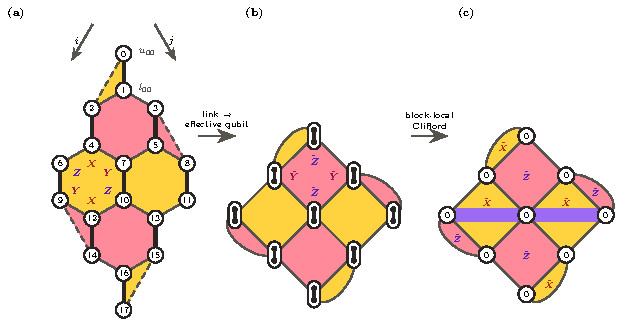
\includegraphics[width=0.86\textwidth]{fig_code.pdf}
  \caption{The distance-3 $XYZ^2$ code. (a)~The 18 qubits sit on the vertices of a honeycomb patch. Thick vertical edges are the nine $XX$ links. Block $(0,0)$ is the top link, with upper vertex $u_{00}$ and lower vertex $l_{00}$, and the indices $i$ and $j$ grow toward the lower left and the lower right. The four shaded hexagons and the four dashed triangles are the weight-six and weight-three plaquette checks. The Pauli labels on hexagon $H_{10}$ show the pattern $XYZXYZ$ of \autoref{eq:hexagon}. Coral cells have $i+j$ even (class B) and sunflower cells have $i+j$ odd (class A). (b)~Each link is a $[[2,1,1]]$ code that holds one effective qubit. On the $3\times3$ array of effective qubits every plaquette acts as $\eff{Z}$ on two diagonally opposite blocks and as $\eff{Y}$ on the other two, which defines the YZZY surface code. (c)~The block-local Clifford map of \autoref{sec:frame} turns the YZZY code into a CSS surface code, with $\eff{Z}$-type class-B plaquettes and $\eff{X}$-type class-A plaquettes. The logical operator $\Xb$ (violet band) becomes a $\eff{Z}$-type string, and $\plusL$ becomes the logical zero state, which is prepared from effective zero states.}
  \label{fig:code}
\end{figure*}

The logical operator
\begin{equation}
  \Xb=\prod_{i+j=d-1}X_{l_{ij}}
  \label{eq:xbar}
\end{equation}
acts on the lower vertices of the $d$ blocks on the anti-diagonal $i+j=d-1$, which form the middle row of the patch. It has weight $d$ and contains only $X$ operators. The operators $\Yb$ and $\Zb$ mix Pauli types~\cite{Sri2022}. \autoref{fig:logicals} shows the three logical operators for $d=3$. In this paper we prepare $\plusL$, the $+1$ eigenstate of $\Xb$. Only errors that anticommute with $\Xb$ can corrupt this state. For the distances studied here, the lightest logical operator that anticommutes with $\Xb$ has weight $d+1$, as $\Yb$ does in \autoref{fig:logicals}(b). The preparation of $\plusL$ is therefore protected to distance $d+1$, one more than the code distance.

\begin{figure}[t]
  \centering
  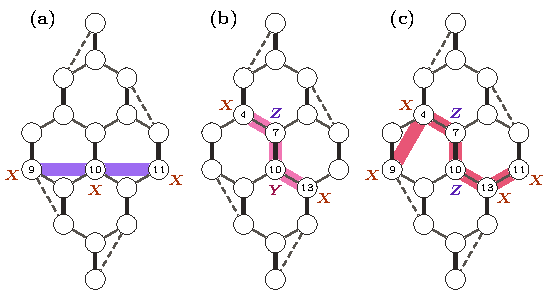
\includegraphics[width=\columnwidth]{fig_logicals.pdf}
  \caption{Logical operators of the $d=3$ code. (a)~$\Xb=X_9X_{10}X_{11}$ has weight 3. (b)~$\Yb=X_4Z_7Y_{10}X_{13}$ has weight 4. (c)~$\Zb=X_4Z_7X_9Z_{10}X_{11}X_{13}$ is the product of $\Xb$ and $\Yb$ up to a phase.}
  \label{fig:logicals}
\end{figure}

\subsection{Block structure}
\label{sec:blocks}

Each block carries a $[[2,1,1]]$ phase-flip code with stabilizer $L_{ij}$. We take
\begin{equation}
  \eff{Z}_{ij}=X_{u_{ij}},\qquad \eff{X}_{ij}=Z_{u_{ij}}Z_{l_{ij}}
\end{equation}
as its logical operators, so that $\eff{Y}_{ij}\propto Y_{u_{ij}}Z_{l_{ij}}$, which equals $Z_{u_{ij}}Y_{l_{ij}}$ up to a sign and a factor of $L_{ij}$. Multiplying a hexagon by links does not change the code. Up to such factors, every hexagon acts on its four blocks as
\begin{equation}
  H_{ij}\simeq \eff{Z}_{i,j}\,\eff{Y}_{i,j+1}\,\eff{Z}_{i+1,j+1}\,\eff{Y}_{i+1,j}.
  \label{eq:yzzy}
\end{equation}
The blocks therefore carry a $d\times d$ surface code with YZZY plaquettes, and the boundary checks become its weight-two boundary stabilizers [\autoref{fig:code}(b)]. The $XYZ^2$ code is this YZZY surface code concatenated with the $d^2$ link codes~\cite{Sri2022,Sri2025}.

We call block $(i,j)$ even if $i+j$ is even and odd otherwise. The same parity splits the cells into two classes. A class-B cell ($i+j$ even) acts as $\eff{Z}$ on two even blocks and as $\eff{Y}$ on two odd blocks. A class-A cell ($i+j$ odd) acts as $\eff{Z}$ on two odd blocks and as $\eff{Y}$ on two even blocks. The boundary checks on the upper-right and lower-left edges belong to class B and those on the upper-left and lower-right edges to class A. This bipartition plays the role of the $X$ and $Z$ plaquettes of the CSS surface code in \autoref{sec:protocol}.

The concatenated structure also explains how errors appear in the syndrome. A $Z$ error on either vertex of block $(i,j)$ flips $L_{ij}$. The two errors differ by $\eff{X}_{ij}$, so the link syndrome reveals that the block was hit but not which vertex. The sequential decoder of Ref.~\cite{Sri2025} removes every link syndrome with a fixed choice of vertex and passes the resulting conditional error probabilities of the effective qubits to a decoder of the YZZY code. We return to this two-level structure in \autoref{sec:decoding}.

\section{Measurement, decoding and recovery}
\label{sec:mdr}

\subsection{Projective preparation}
\label{sec:mdr_basic}

Let $\mathcal{S}$ be the stabilizer group of the code and let $\mathcal{G}=\{G_1,\dots,G_m\}$ be a set of commuting Pauli operators whose joint $+1$ eigenspace is one dimensional. For $\plusL$ we take the $2d^2-1$ stabilizer generators together with $\Xb$, so that
\begin{equation}
  \plusL\!\bra{\bar{+}}=\prod_{k=1}^{m}\Pi_k^{+},\qquad \Pi_k^{\pm}=\tfrac{1}{2}\left(I\pm G_k\right).
  \label{eq:target}
\end{equation}
Measurement, decoding and recovery (MDR) prepares this state as follows:
\begin{enumerate}
  \item Prepare the data qubits in a product state $\ket{\psi_0}$.
  \item Measure every $G_k$ with an ancilla, which gives an outcome $s_k\in\{0,1\}$.
  \item Decode the outcomes into a Pauli recovery $R$.
  \item Apply $R$, or record it in the Pauli frame.
\end{enumerate}
\autoref{fig:mdr}(a) shows the measurement of a single operator $G$. The ancilla starts in $\ket{0}$ and the first Hadamard gate prepares $\ket{+}$. The controlled-$G$ gate then maps
\begin{align}
  \ket{+}\ket{\psi}\;&\mapsto\;\tfrac{1}{\sqrt{2}}\big(\ket{0}\ket{\psi}+\ket{1}G\ket{\psi}\big)\nonumber\\
  &=\ket{+}\,\Pi^{+}\ket{\psi}+\ket{-}\,\Pi^{-}\ket{\psi}.
  \label{eq:projection}
\end{align}
The second Hadamard gate and the measurement in the $Z$ basis read out the ancilla in the $X$ basis. The outcome $s$ occurs with probability $\|\Pi^{(-1)^s}\ket{\psi}\|^2$ and leaves the data in the state $\Pi^{(-1)^s}\ket{\psi}$, up to normalization. To undo the outcome $s=1$ we choose a toggle $P$, a Pauli operator that anticommutes with $G$ and commutes with every other element of $\mathcal{G}$. It satisfies
\begin{equation}
  P\,\Pi^{-}=\Pi^{+}P,
  \label{eq:toggle}
\end{equation}
so the classically controlled gate $P^{s}$ moves the data into the $+1$ eigenspace of $G$ without disturbing the other eigenvalues. For $\Xb$ the toggle is a logical operator that anticommutes with $\Xb$, for example $\Yb$. Without noise the recovery
\begin{equation}
  R=\prod_{k=1}^{m}P_k^{s_k}
  \label{eq:recovery}
\end{equation}
maps the post-measurement state to $\plusL$ for every set of outcomes. In the circuits of this paper each ancilla is prepared directly in $\ket{+}$ and measured in the $X$ basis, which removes the two Hadamard gates, and every recovery is applied in the Pauli frame.

\begin{figure*}[t]
  \centering
  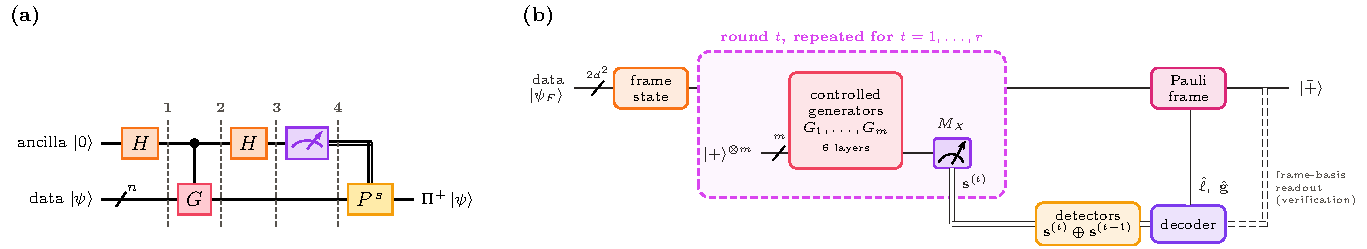
\includegraphics[width=\textwidth]{fig_mdr.pdf}
  \caption{MDR circuits. (a)~Measurement of one operator $G$ with feedforward. (1)~The Hadamard gate prepares the ancilla in $\ket{+}$. (2)~The controlled-$G$ gate entangles the ancilla with the data as in \autoref{eq:projection}. (3)~The second Hadamard gate maps the $X$ basis of the ancilla to the $Z$ basis. (4)~The outcome $s$ controls the toggle $P$, which anticommutes with $G$, and the data end in the $+1$ eigenspace of $G$. (b)~The fault-tolerant protocol of \autoref{sec:protocol}. The $2d^2$ data qubits start in the frame state $\ket{\psi_F}$. Each round measures all $m=2d^2-1$ generators with $m$ ancillas in $\ket{+}$, six layers of controlled Pauli gates and $X$-basis measurements. The outcomes $\mathbf{s}^{(t)}$ of consecutive rounds are combined into detectors. The decoder processes all rounds at once and returns the logical bit $\hat\ell$ and the gauge toggles $\hat{\mathbf{g}}$, which update the Pauli frame. The dashed path is the destructive readout in the frame basis that we use to verify the prepared state.}
  \label{fig:mdr}
\end{figure*}

\subsection{Deterministic checks and fault distance}
\label{sec:s0}

With noise the outcomes $s_k$ are not reliable. A data error before a measurement changes the outcome of every generator that anticommutes with it, and a measurement error changes a single outcome. The decoder has to tell these apart, and it can only do so with outcomes whose values are known in advance. Before the first round the data qubits are in the state $\ket{\psi_0}$. We define
\begin{equation}
  \Sz=\left\{S\in\mathcal{S}\;:\;S\ket{\psi_0}=\pm\ket{\psi_0}\right\}
  \label{eq:S0}
\end{equation}
as the group of stabilizers whose values are fixed by the initial state. The subscript $0$ refers to round zero, the state before any measurement. Without faults, the value of an element of $\Sz$ in the first round equals its value on $\ket{\psi_0}$, and every later value equals the one before. A generator of $\mathcal{S}$ outside $\Sz$ has a uniformly random first outcome, and only its changes from one round to the next are deterministic. We call these generators gauge generators, because their random values are absorbed into the Pauli frame and carry no logical information.

A detector is a parity of outcomes that is deterministic in the absence of faults. Let $s_S^{(t)}\in\{0,1\}$ be the measured value of a stabilizer $S$ in round $t$, which for a product of generators is the parity of their outcomes, and let $s_S^{(0)}$ be the known value of an element of $\Sz$ on $\ket{\psi_0}$. The detectors of the $r$ rounds are
\begin{equation}
  D_S^{(t)}=s_S^{(t)}\oplus s_S^{(t-1)},
  \label{eq:detectors}
\end{equation}
with $t=1,\dots,r$ for the generators of $\Sz$ and $t=2,\dots,r$ for the gauge generators.
An error that occurs before the first measurement of a generator is visible only in a detector with $t=1$, and these exist only for $\Sz$. The choice of $\ket{\psi_0}$ therefore decides which early errors can be detected.

We quantify this with the circuit-level fault distance. An elementary fault is a Pauli error after a gate, a preparation or an idle step, or a flipped measurement outcome. The detector error model (DEM) of a circuit lists every elementary fault $j$ with its probability $p_j$, the detectors it flips and whether it flips the logical observable~\cite{gidney2021stim}. We write the detectors of fault $j$ as the column $H_j$ of a binary matrix $H$ and its effect on the observable as the entry $L_j$ of a binary row vector $L$. A set of faults, written as a binary vector $x$, is an undetectable logical error if
\begin{equation}
  Hx=0\pmod 2,\qquad Lx=1\pmod 2.
  \label{eq:undetectable}
\end{equation}
The fault distance $d_f$ is the smallest Hamming weight of such an $x$. A decoder that corrects every set of fewer than $d_f/2$ faults then has a logical error rate
\begin{equation}
  \pL=O\big(p^{\lceil d_f/2\rceil}\big)
  \label{eq:scaling}
\end{equation}
at small physical error rate $p$. For $\plusL$ the largest possible value is $d_f=d+1$, the weight of the lightest logical operator that anticommutes with $\Xb$ (\autoref{sec:code}).

The simplest product state on which $\Xb$ is deterministic is $\ket{+}^{\otimes n}$. On this state $\Sz$ is generated by the $d^2$ links. A $Z$ error on either vertex of a block flips the same link, but on an anti-diagonal block only the error on the lower vertex flips $\Xb$ [\autoref{fig:frame}(a)]. Two preparation errors $Z_{u_{ij}}Z_{l_{ij}}$ on such a block commute with every link and anticommute with $\Xb$. They change only the random first outcomes of the hexagons, so the two faults form an undetectable logical error. The $\ket{+}^{\otimes n}$ start therefore has fault distance two at every $d$, whatever circuit and decoder follow it (\autoref{tab:fd}). The protocol of the next section chooses $\ket{\psi_0}$ so that $\Sz$ separates these errors.

\section{Fault-tolerant MDR}
\label{sec:protocol}

The fault-tolerant protocol keeps the structure of MDR but changes each of its steps. It prepares $\plusL$ as follows (\autoref{fig:protocol}):
\begin{enumerate}
  \item \emph{Prepare.} Initialize every data qubit in a single-qubit state chosen in the CSS frame of the code. The operator $\Xb$ and the group $\Sz$ of \autoref{eq:S0}, which then has $d^2$ independent generators, are deterministic.
  \item \emph{Measure.} Measure all $2d^2-1$ generators for $r$ rounds with one ancilla per generator and a depth-six interleaved schedule. The logical operator is never measured directly.
  \item \emph{Decode.} Decode the full space-time detector history after the last round.
  \item \emph{Recover.} Update the Pauli frame with the logical bit returned by the decoder and with the toggles of the generators whose first outcomes are random.
\end{enumerate}
We describe the four steps below and then give the fault distance.

\begin{figure*}[t]
  \centering
  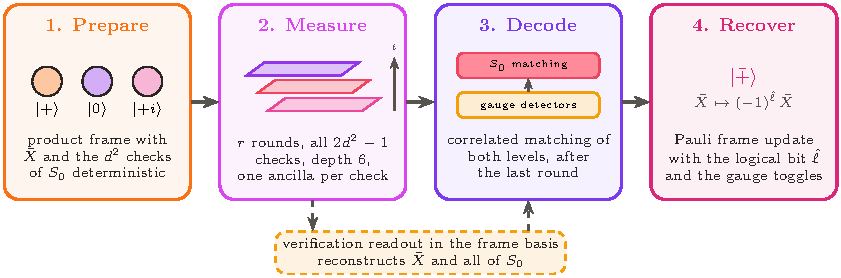
\includegraphics[width=\textwidth]{fig_protocol.pdf}
  \caption{The fault-tolerant MDR protocol. (1)~Every data qubit is prepared in a single-qubit eigenstate of its frame Pauli, which fixes $\Xb$ and the $d^2$ elements of $\Sz$. (2)~All $2d^2-1$ generators are measured for $r$ rounds with one ancilla each. (3)~A decoder processes the detectors of all rounds at once. In hierarchical correlated matching the gauge detectors form a lower level that reweights the matching of the $\Sz$ detectors. (4)~The recovery is a Pauli frame update. For verification on hardware the data qubits are read out destructively in the frame basis, which reconstructs $\Xb$ and every element of $\Sz$.}
  \label{fig:protocol}
\end{figure*}

\subsection{Frame initialization}
\label{sec:frame}

The YZZY surface code of \autoref{sec:blocks} becomes a CSS code under a block-local Clifford map. On even blocks we keep $\eff{Z}$ and map $\eff{Y}\mapsto\eff{X}$. On odd blocks we map $\eff{Y}\mapsto\eff{Z}$ and $\eff{Z}\mapsto\eff{X}$. By \autoref{eq:yzzy}, every class-B plaquette becomes $\eff{Z}^{\otimes4}$ and every class-A plaquette becomes $\eff{X}^{\otimes4}$. The logical operator $\Xb$ acts as $\eff{Z}$ on the even blocks of the anti-diagonal, so it becomes a $Z$-type logical operator. In this frame $\plusL$ corresponds to the logical zero state of a CSS surface code, which is prepared fault tolerantly from the product state of effective zero states [\autoref{fig:code}(c)]. Mapping back to the $XYZ^2$ code, every even block has to be a $+1$ eigenstate of $\eff{Z}=X_u$ and every odd block a $+1$ eigenstate of $\eff{Y}\simeq Z_uY_l$.

We realize these effective eigenstates with the single-qubit product state
\begin{equation}
  \ket{\psi_F}=\bigotimes_{i+j\ \mathrm{even}}\ket{+}_{u_{ij}}\ket{+}_{l_{ij}}\;\otimes\bigotimes_{i+j\ \mathrm{odd}}\ket{0}_{u_{ij}}\ket{{+}i}_{l_{ij}}.
  \label{eq:frame}
\end{equation}
Every data qubit is thus an eigenstate of one frame Pauli, $X$ on both vertices of an even block, $Z$ on the upper and $Y$ on the lower vertex of an odd block. \autoref{fig:frame}(c) shows this frame for $d=5$. The even blocks are also eigenstates of their links. The odd blocks are not, because a state of the $[[2,1,1]]$ code with a definite value of $\eff{Y}$ is entangled. We accept this and keep the initialization free of entangling gates.

A stabilizer has a definite value on $\ket{\psi_F}$ exactly when it is a product of frame Paulis, so $\Sz$ of \autoref{eq:S0} is the set of such stabilizers. For the frame state it has $d^2$ independent generators, namely the $(d^2+1)/2$ even links, the $(d-1)^2/2$ class-B hexagons and the $d-1$ class-B boundary checks. Some of these generators are multiplied by an odd link so that they become products of frame Paulis. For $d=3$, for example, the class-B hexagon $H_{00}$ enters $\Sz$ as $H_{00}L_{01}=X_1Z_2Z_3Y_4Y_5X_7$. The remaining $d^2-1$ generators are the odd links, the class-A hexagons and the class-A boundary checks. These are the gauge generators, whose first outcomes are random. The operator $\Xb$ of \autoref{eq:xbar} acts on lower vertices of even blocks, so it is also a product of frame Paulis and has the value $+1$ on $\ket{\psi_F}$.

Every single-qubit error on the frame state either acts trivially or flips one or two elements of $\Sz$. \autoref{fig:frame} compares this with the $\ket{+}^{\otimes n}$ start. There, $Z$ errors on the two vertices of a block flip only the shared link. In the frame state the same two errors flip different class-B hexagons, so the decoder can tell which of them flipped $\Xb$. The smallest set of single-qubit errors that flips $\Xb$ without flipping any element of $\Sz$ has weight $d+1$.

At the end of the protocol we read out the data qubits destructively in the same frame. Even blocks are measured in the $X$ basis, the upper vertex of every odd block in the $Z$ basis and the lower vertex in the $Y$ basis. These outcomes reconstruct $\Xb$ and every element of $\Sz$, so the final comparison also has distance $d+1$. This readout is used to verify the prepared state. In a computation it is replaced by the next logical operation.

\begin{figure}[t]
  \centering
  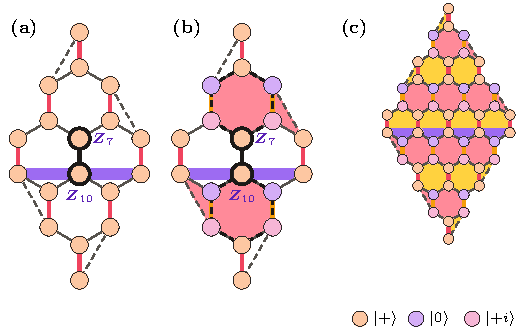
\includegraphics[width=\columnwidth]{fig_frame.pdf}
  \caption{Initial states. Qubit colors give the single-qubit basis ($X$ orange, $Y$ pink, $Z$ purple) and the violet band marks $\Xb$. (a)~Start from $\ket{+}^{\otimes n}$. Only the links (coral) and $\Xb$ are deterministic. The errors $Z_7$ and $Z_{10}$ (black rings) flip the same link (black), but only $Z_{10}$ flips $\Xb$. (b)~Frame start $\ket{\psi_F}$. The coral even links and the coral hexagons belong to $\Sz$. $Z_7$ flips the hexagon $H_{00}L_{01}$ and $Z_{10}$ flips $H_{11}L_{12}$ (dashed outlines), so the two errors are distinguishable. The dashed sunflower links are odd links, which are gauge generators with random first outcomes. (c)~The frame for $d=5$, with class-B cells in coral and class-A cells in sunflower.}
  \label{fig:frame}
\end{figure}

\subsection{Syndrome extraction}
\label{sec:schedule}

Each generator has its own ancilla. One round of extraction consists of the following steps:
\begin{enumerate}
  \item prepare every ancilla in $\ket{+}$,
  \item apply six layers of controlled-Pauli gates, in which each ancilla controls the Pauli of its check on one data qubit,
  \item measure every ancilla in the $X$ basis.
\end{enumerate}
A hexagon ancilla takes part in all six layers, a boundary ancilla in three and a link ancilla in two. Every data qubit takes part in at most one gate per layer. \autoref{fig:schedule}(a) shows the circuit for one hexagon.

The order of the gates matters in two ways. First, interleaved circuits measure the intended operators only if every pair of overlapping checks is compatible. On the shared qubits where two checks $a$ and $b$ apply anticommuting Paulis, the number of qubits on which $a$ acts before $b$ must be even. Second, a fault on an ancilla in the middle of its check spreads to the data qubits that the ancilla touches later. These hook errors can lower the circuit-level distance~\cite{dennis2002,tomita2014}.

We restrict to translation-invariant schedules, in which the layer of each hexagon vertex depends only on its position in the hexagon and on the class of the cell, and the link gates use fixed layers. Boundary checks inherit the layers of their cells. We enumerated every such schedule of depth six that satisfies the compatibility condition and found 8928 of them. For each one we computed the circuit-level fault distance of the $d=3$ protocol with three rounds. 3968 schedules reach distance 2, 3834 reach 3 and 1126 reach the maximum of 4 [\autoref{fig:schedule}(d)]. We chose one of the 1126 and verified that it reaches $d+1$ at $d=5$ and $d=7$. In this schedule a class-A hexagon visits its vertices in the order top, upper left, upper right, lower left, lower right, bottom. A class-B hexagon uses the order top, upper right, lower right, bottom, upper left, lower left. A link ancilla acts on the upper vertex in the first layer and on the lower vertex in the second [\autoref{fig:schedule}(b,c)].

\begin{figure}[t]
  \centering
  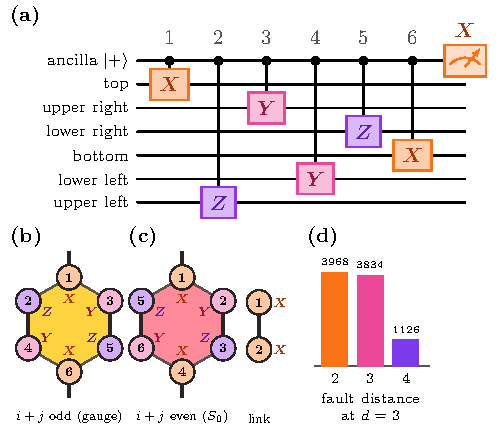
\includegraphics[width=\columnwidth]{fig_schedule.pdf}
  \caption{Syndrome extraction. (a)~Circuit for a class-A hexagon. The ancilla controls the Pauli of the check on each vertex, in the layer given at the top. (b)~Layer in which each vertex of a class-A hexagon is visited, with qubits colored by the Pauli of the check. (c)~The same for class-B hexagons and for links. (d)~Circuit-level fault distance of all 8928 compatible translation-invariant depth-six schedules at $d=3$. The violet bar contains the schedule used here.}
  \label{fig:schedule}
\end{figure}

\subsection{Detectors}
\label{sec:detectors}

The detectors of \autoref{eq:detectors} fall into two families (\autoref{fig:detectors}):
\begin{enumerate}
  \item \emph{$\Sz$ detectors.} For each of the $d^2$ generators of $\Sz$ we compare its value in round 1 with its known initial value and its value in round $t$ with round $t-1$. The destructive readout reconstructs every element of $\Sz$, and we compare it with round $r$. This gives $d^2(r+1)$ detectors.
  \item \emph{Gauge detectors.} The $d^2-1$ gauge generators have random outcomes in round 1. From round 2 onward we compare each with its previous value, which gives $(d^2-1)(r-1)$ detectors. The frame readout does not reconstruct these generators, so they have no final detector.
\end{enumerate}
The observable is the value of $\Xb$ in the frame readout,
\begin{equation}
  \ell=\bigoplus_{i+j=d-1} m_{l_{ij}},
  \label{eq:observable}
\end{equation}
where $m_q\in\{0,1\}$ is the outcome of the $X$-basis readout of qubit $q$. After Stim decomposes each fault into graphlike components, every component flips at most two $\Sz$ detectors~\cite{gidney2021stim}. The $\Sz$ detectors alone therefore define a matching graph, in the same way as the $Z$-type detectors of a CSS surface code. The gauge detectors add information that a matching decoder on $\Sz$ ignores. We use them in \autoref{sec:decoding}. For $r=1$ there are no gauge detectors.

\begin{figure}[t]
  \centering
  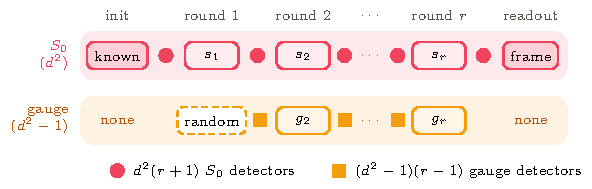
\includegraphics[width=\columnwidth]{fig_detectors.pdf}
  \caption{Detectors of the protocol. Columns are the initial state, the $r$ extraction rounds and the frame readout. Each coral dot compares the $d^2$ generators of $\Sz$ between two neighboring columns. Each sunflower square compares the $d^2-1$ gauge generators between two neighboring rounds. The gauge generators are random in round 1 and are not reconstructed by the readout.}
  \label{fig:detectors}
\end{figure}

\subsection{Decoding and recovery}
\label{sec:recovery}

The decoder receives the detection events of all rounds and returns one bit $\hat\ell$, the prediction of whether the observable $\Xb$ was flipped. We correct the readout of $\Xb$ with this bit, and a shot is a logical failure if the corrected value differs from $+1$. The logical error rate is therefore
\begin{equation}
  \pL=\Pr\big[\ell\oplus\hat\ell=1\big].
  \label{eq:pL}
\end{equation}
When the state is not read out, the bit is applied as a logical Pauli frame update, together with the toggles of the gauge generators whose round-1 outcomes were $-1$. These toggles commute with $\Xb$ and with $\Sz$, so they do not affect the logical value. Pauli frame updates are applied in software, and a physical correction is only needed before a non-Clifford gate~\cite{knill2005,gottesman1998}. The baseline decoder is minimum-weight perfect matching (MWPM) on the $\Sz$ detectors~\cite{dennis2002,higgott2025sparse}. The decoders that also use the gauge detectors are the subject of \autoref{sec:decoding}.

The protocol is decoded once, after the last round, so that a measurement error in one round and a data error are told apart by the rounds around them. In a computation the last round of preparation is decoded together with the rounds of error correction that follow it. To score the prepared state on its own, we end the circuit either with the destructive frame readout or with one noiseless round of all generators and $\Xb$, which we call the ideal readout.

\subsection{Fault distance}
\label{sec:fd}

We computed the circuit-level fault distance of the protocol exactly by solving the minimum-weight problem of \autoref{eq:undetectable} on the detector error model (Appendix~\ref{app:distance}). For $d=3$ and $5$, with $r=1$ and $r=d$ rounds and either readout, and for $d=7$ with one round, the minimum number of faults that flips $\Xb$ without triggering an $\Sz$ detector is $d+1$ (\autoref{tab:fd}). For $d=7$ with seven rounds a linear-programming bound shows that every undetectable logical error contains at least seven faults, and the undetectable-error search of Stim finds one with eight. The protocol is therefore fault tolerant with the full distance available for $\plusL$, and the extraction circuit does not lose distance to hook errors. The $\ket{+}^{\otimes n}$ start with the same schedule and all detectors has fault distance two at every $d$, which confirms that the initial state, and not the circuit, limits that variant.

\begin{table}[t]
  \caption{Circuit-level fault distance for the preparation of $\plusL$. The values of the fault-tolerant protocol hold for $r=1$ and $r=d$ rounds and for the destructive or the ideal final readout. They are exact for $d=3$ and $5$ and for $d=7$ with one round (Appendix~\ref{app:distance}). For $d=7$ with seven rounds we prove that the fault distance is at least seven, and the search of Stim finds an undetectable logical error with eight faults.}
  \label{tab:fd}
  \begin{ruledtabular}
  \begin{tabular}{lccc}
    Initial state & $d=3$ & $d=5$ & $d=7$ \\
    \hline
    $\ket{+}^{\otimes n}$, all detectors & 2 & 2 & 2 \\
    Frame state $\ket{\psi_F}$, $\Sz$ detectors & 4 & 6 & 8 \\
  \end{tabular}
  \end{ruledtabular}
\end{table}

\section{Decoders}
\label{sec:decoding}

All decoders start from the detector error model of \autoref{sec:s0}. Fault $j$ has the prior probability $p_j$ and the log-likelihood ratio $\lambda_j=\ln[(1-p_j)/p_j]$, flips the detectors in the column $H_j$ and flips the observable if $L_j=1$. Given the detection events $\sigma$ of a shot, the most likely set of faults is
\begin{equation}
  \hat{x}=\arg\min_{x\,:\,Hx=\sigma}\ \sum_j\lambda_j x_j,\qquad \hat\ell=L\hat{x}\pmod 2 .
  \label{eq:mle}
\end{equation}
The first six decoders approximate \autoref{eq:mle} in different ways, and the coset free-energy decoder of \autoref{sec:cfe} compares the probabilities of the two logical classes instead. In our protocol most faults flip $\Sz$ detectors and gauge detectors together. A $Z$ error on a qubit of an even block, for example, flips an even link and a class-B hexagon in $\Sz$ and also a class-A hexagon among the gauge generators. The baseline matching decoder discards the gauge half of this information, and the other decoders differ in how they use it. \autoref{fig:decoderzoo} illustrates each decoder and \autoref{tab:decoders} summarizes them.

\begin{figure*}[t]
  \centering
  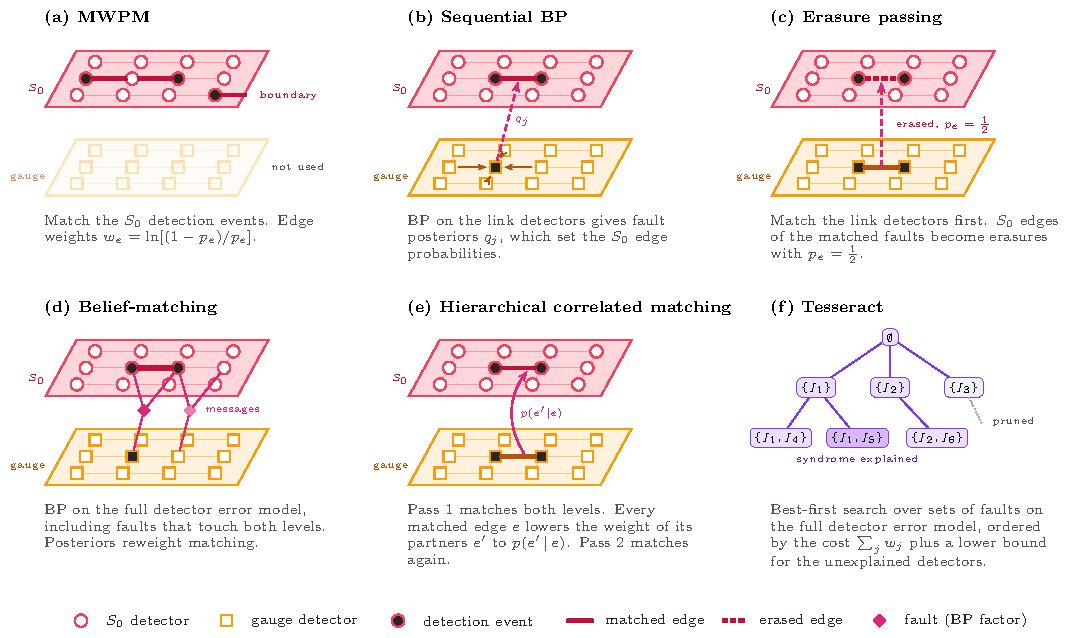
\includegraphics[width=\textwidth]{fig_decoder_zoo.pdf}
  \caption{The decoders of this paper. In every panel the upper plane is the matching graph of the $\Sz$ detectors (coral circles) and the lower plane is the graph of the gauge detectors (sunflower squares), each drawn for a few detectors in space and time. Filled symbols are detection events. (a)~MWPM matches the $\Sz$ detection events with the weights of \autoref{eq:weights} and ignores the gauge level. (b)~Sequential BP runs belief propagation on the link detectors, and the fault posteriors $q_j$ set the probabilities of the $\Sz$ edges through \autoref{eq:posterior_edges}. (c)~Erasure passing matches the link detectors and erases the $\Sz$ edges of the faults with a matched link signature. (d)~Belief-matching runs belief propagation on the full detector error model. Each fault (diamond) connects detectors of both levels, and its posterior reweights the matching on $\Sz$. (e)~Hierarchical correlated matching matches both levels, raises the probability of every edge that shares a fault with a matched edge to the conditional probability of \autoref{eq:conditional} and matches again. (f)~Tesseract searches over sets of faults on the full detector error model and expands the cheapest partial solution first.}
  \label{fig:decoderzoo}
\end{figure*}

\subsection{Matching on the frame-deterministic detectors}

Stim decomposes every fault into graphlike components, each of which flips at most two $\Sz$ detectors~\cite{gidney2021stim}. These components are the edges $e$ of a matching graph, with a boundary vertex for components that flip a single detector. If the faults $j$ that contain edge $e$ act independently, the edge is flipped with probability
\begin{equation}
  p_e=\frac12\Big[1-\prod_{j\ni e}\left(1-2p_j\right)\Big],\qquad w_e=\ln\frac{1-p_e}{p_e},
  \label{eq:weights}
\end{equation}
and \autoref{eq:mle} restricted to the $\Sz$ detectors becomes a minimum-weight perfect matching problem,
\begin{equation}
  E^\star=\arg\min_{E\,:\,\partial E=\sigma_0}\ \sum_{e\in E}w_e,\qquad \hat\ell=\bigoplus_{e\in E^\star}L_e .
  \label{eq:mwpm}
\end{equation}
Here $\sigma_0$ is the set of $\Sz$ detection events, $\partial E$ is the set of vertices that meet an odd number of edges of $E$, and $L_e$ records whether edge $e$ flips the observable. We use the sparse blossom implementation in PyMatching~\cite{higgott2025sparse,higgott2022pymatching}. This decoder has the full fault distance of \autoref{sec:fd} and costs about $7\,\mu$s per shot at $d=5$ [\autoref{fig:decoderzoo}(a)].

\subsection{Sequential decoding with soft information}
\label{sec:seqbp}

The sequential decoder of Srivastava \emph{et al.}~\cite{Sri2025} first decodes the $[[2,1,1]]$ link codes and then passes conditional error probabilities of the effective qubits to a decoder of the YZZY code. In a circuit the link syndromes are themselves noisy and are spread over many rounds, so we use a circuit-level analogue. We first run belief propagation (BP) on the part of the DEM that contains the link detectors, both the even links in $\Sz$ and the odd links among the gauge detectors~\cite{roffe2020}. BP passes messages between faults $j$ and detectors $i$ on the Tanner graph of $H$,
\begin{align}
  \mu_{j\to i}&=\lambda_j+\sum_{i'\in N(j)\setminus i}\nu_{i'\to j},\label{eq:bp_v}\\
  \nu_{i\to j}&=(-1)^{\sigma_i}\,2\,\mathrm{artanh}\!\prod_{j'\in N(i)\setminus j}\tanh\frac{\mu_{j'\to i}}{2},\label{eq:bp_c}
\end{align}
where $N(\cdot)$ denotes the neighbors in the Tanner graph. After 30 iterations of the product-sum rule the posterior log-likelihood ratio of fault $j$ is $\Lambda_j=\lambda_j+\sum_{i\in N(j)}\nu_{i\to j}$, and its posterior probability is $q_j=1/(1+e^{\Lambda_j})$. We convert these posteriors into probabilities of the $\Sz$ edges,
\begin{equation}
  p_e=1-\prod_{j\,:\,e\in j}\left(1-q_j\right),
  \label{eq:posterior_edges}
\end{equation}
where the product runs over the faults whose decomposition contains $e$, and we match on $\Sz$ with the weights $w_e$ of these per-shot probabilities [\autoref{fig:decoderzoo}(b)]. We call this decoder sequential BP.

\subsection{Erasure passing}

A hard-decision version of the same idea passes erasures from the lower level to the upper level [\autoref{fig:decoderzoo}(c)]. We match the link detection events on their own graph. Every fault whose link signature equals a matched link edge is marked, and all $\Sz$ edges of the marked faults receive
\begin{equation}
  p_e=\tfrac12,\qquad w_e=0 .
  \label{eq:erasure}
\end{equation}
Matching on $\Sz$ then treats these edges as erased, since a path through them costs nothing~\cite{stace2009}. This decoder uses the same information as sequential BP but replaces probabilities by flags.

\subsection{Belief-matching}

Belief-matching runs BP with \autoref{eq:bp_v} and \autoref{eq:bp_c} on the full DEM, with every $\Sz$ and gauge detector, and reweights the matching graph with \autoref{eq:posterior_edges}~\cite{higgott2023}. A fault that flips detectors of both levels is a single variable node of the Tanner graph [\autoref{fig:decoderzoo}(d)], so BP propagates the gauge syndrome to the $\Sz$ edges directly. It is the soft-information decoder with the most complete input.

\subsection{Hierarchical correlated matching}
\label{sec:hcm}

Our decoder keeps the two-level structure but uses matching at both levels (\autoref{fig:decoder}). The upper level is the $\Sz$ graph, which decides the logical outcome. The lower level is the graph of the gauge detectors, which contains the odd links, the class-A hexagons and the class-A boundary checks. We build a DEM in which each fault is split into an upper part and a lower part as follows:
\begin{enumerate}
  \item The upper part is the set of graphlike $\Sz$ components of the fault, with the observable, as in the matching decoder.
  \item The lower part is the set of gauge detectors that the fault flips, decomposed into edges of the lower graph. Faults whose lower part cannot be decomposed keep only their upper part.
  \item The two parts are joined into one correlated error mechanism with the probability of the fault.
\end{enumerate}
We decode this model with the two-pass correlated matching of PyMatching~\cite{fowler2013,higgott2025sparse}. The first pass solves \autoref{eq:mwpm} on both levels with the prior weights. For every edge $e$ in the first solution and every edge $e'$ that occurs together with $e$ in some fault, the second pass replaces the weight of $e'$ by that of the conditional probability
\begin{equation}
  p(e'\,|\,e)=\frac{\Pr[e\text{ and }e'\text{ flipped by one fault}]}{\Pr[e\text{ flipped}]},
  \label{eq:conditional}
\end{equation}
and then matches again [\autoref{fig:decoderzoo}(e)]. A matched lower edge thus tells the upper level which of its edges are likely, which is the role of the link syndromes in sequential decoding. Unlike sequential decoding, the information flows in both directions and both levels are solved by matching.

\begin{figure*}[t]
  \centering
  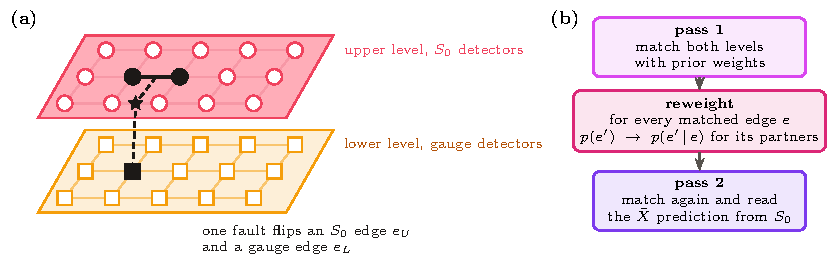
\includegraphics[width=0.8\textwidth]{fig_decoder.pdf}
  \caption{Hierarchical correlated matching. (a)~The upper level is the matching graph of the $\Sz$ detectors and the lower level the graph of the gauge detectors. A single fault (star) flips an edge $e_U$ of the upper graph and an edge $e_L$ of the lower graph, so the two levels are correlated. (b)~Two-pass correlated matching. The first pass matches both levels with prior weights. The second pass raises the probability of every edge that shares a fault with a matched edge to the conditional probability of \autoref{eq:conditional}, matches again and reads the prediction for $\Xb$ from the upper level.}
  \label{fig:decoder}
\end{figure*}

We also consider a variant whose lower level contains only the odd-link detectors. It isolates the contribution of the $[[2,1,1]]$ link codes. We call the full decoder hierarchical correlated matching (HCM) and the variant HCM with links.

\subsection{Tesseract}

As a reference we use Tesseract, a search-based decoder that solves \autoref{eq:mle} on the full DEM, with all detectors, by an A$^\star$ search over sets of faults~\cite{beni2025}. The search expands the partial solution $F$ with the lowest cost $\sum_{j\in F}\lambda_j$ plus a lower bound for the detection events that $F$ leaves unexplained [\autoref{fig:decoderzoo}(f)]. We run it with a detector beam of 20 and beam climbing. It is a near-optimal reference at small distances but is four orders of magnitude slower than matching here.

\subsection{Coset free-energy decoding}
\label{sec:cfe}

Every decoder above, Tesseract included, approximates the most likely error of \autoref{eq:mle}. The prediction, however, depends only on the logical class of the error. The optimal decoder compares the total probabilities of the two classes~\cite{dennis2002,bravyi2014},
\begin{equation}
  Z_\ell=\sum_{x\,:\,Hx=\sigma,\ Lx=\ell}\ \prod_j p_j^{x_j}(1-p_j)^{1-x_j},
  \label{eq:coset}
\end{equation}
and returns $\hat\ell=\arg\max_{\ell}Z_\ell$. The most likely error can lie in the less likely class if the other class contains many more errors of similar weight. Near threshold logical failures are long chains, and the number of such chains matters as much as their weight. We introduce the coset free-energy (CFE) decoder, which estimates the free energies $F_\ell=-\ln Z_\ell$ in three steps (\autoref{fig:cfe}).

\emph{Two-class search.} We append the observable row $L$ to $H$ and run BP followed by ordered-statistics decoding (BP-OSD)~\cite{panteleev2021,roffe2020} once with the target $(\sigma,0)$ and once with $(\sigma,1)$. Each run returns a low-weight error $x_\ell$ with $Hx_\ell=\sigma$ and $Lx_\ell=\ell$. We use 30 iterations of product-sum BP and the combination sweep of order 10. A second pair of runs starts from per-shot priors in which every fault on the HCM solution has probability $0.3$, which gives a second candidate in each class.

\emph{Local descent.} A degeneracy move is a set $g$ of faults with $\sum_{j\in g}H_j=0$ and $\sum_{j\in g}L_j=0$ modulo 2, so that $x\oplus g$ has the same syndrome and the same class as $x$. We use all moves of three faults, in which one fault is the sum of two others, such as a $Y$ error and its $X$ and $Z$ parts, and all moves of four faults, in which two pairs of adjacent faults flip the same detectors, such as the two paths around a square of the decoding graph. At $d=5$ there are $1.9\times10^{5}$ such moves. A move changes the weight $w(x)=\sum_j\lambda_jx_j$ by
\begin{equation}
  \Delta w_g(x)=\sum_{j\in g\setminus x}\lambda_j-\sum_{j\in g\cap x}\lambda_j ,
  \label{eq:dw}
\end{equation}
and we apply the move with the most negative $\Delta w_g$ until no move lowers the weight.

\emph{Free energy.} If the moves that touch $x_\ell$ acted independently, the class would contain $x_\ell\oplus\bigoplus_{g\in G}g$ for every subset $G$ of them, and
\begin{equation}
  F_\ell\approx w(x_\ell)-\kappa\sum_{g\,:\,g\cap x_\ell\neq\emptyset}\ln\!\left(1+e^{-\Delta w_g(x_\ell)}\right)
  \label{eq:cfe}
\end{equation}
with $\kappa=1$. Moves that share faults are not independent, and the sum then counts some errors more than once. A single factor $\kappa<1$ corrects for this on average. We use $\kappa=1/2$ for all noise models. For each class the decoder keeps the candidate with the smaller $F_\ell$ and returns the class with the smaller free energy. With $\kappa=0$ it returns the class of the lighter candidate, which is the most-likely-error rule of \autoref{eq:mle} with a two-class search.

The idea of counting equivalent errors is not new. Multi-path summation adds the number of shortest paths to the matching weights~\cite{criger2018}, and Markov chain Monte Carlo samples the classes directly~\cite{hutter2014}. The CFE decoder works on the full circuit-level DEM, including hyperedges, and needs neither a planar graph nor sampling. Its cost is dominated by the four BP-OSD runs and by the local descent. At $d=5$ it takes $0.23$\,s per shot in our Python implementation, compared with $0.14$\,s for Tesseract (\autoref{tab:decoders}). The guided pair matters only when the two classes are close. If it runs only when the free energies of the first pair differ by less than 6, the number of failures changes by at most $2\%$ in our samples and the cost halves.

\begin{figure*}[t]
  \centering
  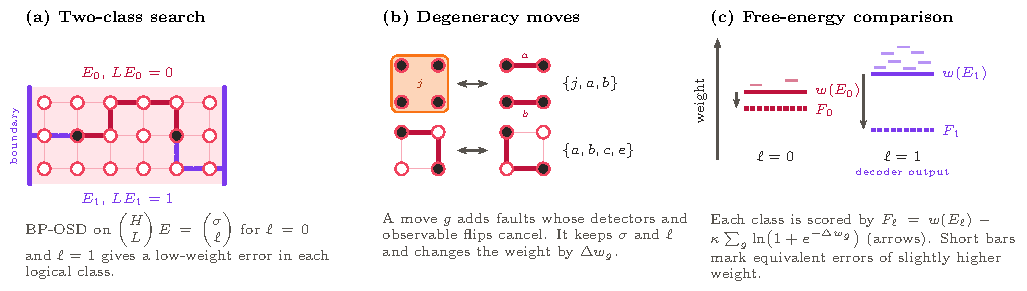
\includegraphics[width=\textwidth]{fig_cfe.pdf}
  \caption{The coset free-energy decoder. (a)~BP-OSD with the observable appended to the check matrix finds a low-weight error in each logical class, here $E_0$ (coral), which pairs the two detection events, and $E_1$ (violet, dashed), which connects them to opposite boundaries. (b)~Degeneracy moves keep the syndrome and the class. A three-fault move replaces a hyperedge $j$ by two edges $a$ and $b$ that flip the same detectors. A four-fault move exchanges the two paths around a square. Greedy moves lower the weight of each candidate. (c)~The free energy subtracts the entropy of the moves around each candidate, \autoref{eq:cfe}. The decoder can then choose the class with the heavier candidate if that class contains many more errors of similar weight.}
  \label{fig:cfe}
\end{figure*}

\begin{table}[t]
  \caption{Decoders and the detectors they use. The decoding time per shot is the CPU time at $d=5$, $r=5$ under SD6 noise with $p=4\times10^{-3}$ on one core. The BP-based decoders and erasure passing rebuild the matching graph for every shot in Python, so their times are upper bounds.}
  \label{tab:decoders}
  \begin{ruledtabular}
  \begin{tabular}{lll}
    Decoder & Detectors & Time per shot \\
    \hline
    MWPM & $\Sz$ & $7\,\mu$s \\
    Sequential BP & links $\to$ $\Sz$ & $7.8$\,ms \\
    Erasure passing & links $\to$ $\Sz$ & $1.0$\,ms \\
    Belief-matching & all $\to$ $\Sz$ & $7.6$\,ms \\
    HCM with links & $\Sz$ $\leftrightarrow$ odd links & $25\,\mu$s \\
    HCM & $\Sz$ $\leftrightarrow$ gauge & $32\,\mu$s \\
    Tesseract & all & $0.14$\,s \\
    CFE & all & $0.23$\,s \\
  \end{tabular}
  \end{ruledtabular}
\end{table}

\section{Circuit-level simulations}
\label{sec:results}

\subsection{Noise models}
\label{sec:noise}

We simulate all circuits with Stim~\cite{gidney2021stim} and estimate each logical error rate from up to $10^{5}$ shots, or until $10^{3}$ logical errors occur, unless stated otherwise. Every noise model attaches Pauli channels to the locations of the circuit (\autoref{fig:noise}). We use the single-qubit and two-qubit depolarizing channels
\begin{align}
  \mathcal{D}_p(\rho)&=(1-p)\,\rho+\frac{p}{3}\sum_{P\in\{X,Y,Z\}}P\rho P,\label{eq:dep1}\\
  \mathcal{D}^{(2)}_p(\rho)&=(1-p)\,\rho+\frac{p}{15}\sum_{P\in\mathcal{P}_2\setminus\{II\}}P\rho P,\label{eq:dep2}
\end{align}
where $\mathcal{P}_2$ is the set of the 16 two-qubit Pauli operators, the general Pauli channel
\begin{equation}
  \mathcal{N}_{\mathbf{p}}(\rho)=\Big(1-\sum_{P\neq I}p_P\Big)\rho+\sum_{P\neq I}p_P\,P\rho P,
  \label{eq:pauli}
\end{equation}
and the flip channel
\begin{equation}
  \mathcal{F}^{Q}_p(\rho)=(1-p)\,\rho+p\,Q\rho Q
  \label{eq:flip}
\end{equation}
of a single Pauli operator $Q$.

Preparation and measurement errors are flips in the basis of the operation. A preparation in the basis $b\in\{X,Y,Z\}$ is followed by $\mathcal{F}^{Q_b}_{p_{\rm r}}$ and a measurement in the basis $b$ is preceded by $\mathcal{F}^{Q_b}_{p_{\rm m}}$, where
\begin{equation}
  Q_X=Z,\qquad Q_Y=X,\qquad Q_Z=X
  \label{eq:flips}
\end{equation}
anticommute with the prepared or measured Pauli [\autoref{fig:noise}(b)]. A flip turns a prepared eigenstate of $b$ into the orthogonal eigenstate and inverts the outcome of a measurement of $b$. A depolarizing channel before a measurement would instead put a third of its probability on the Pauli that commutes with the measured operator, which leaves the outcome unchanged. The ancillas are prepared in $\ket{+}$ and measured in the $X$ basis, so both of their flips are $Z$ errors. The data qubits are prepared and read out in their frame bases, so an even block receives $Z$ flips and an odd block $X$ flips. All simulations in this paper use these basis-dependent flips.

Each round of extraction has six layers of controlled Pauli gates and two steps in which the ancillas are reset or measured. A noise model specifies the channel after every gate, on every qubit that idles in a gate layer, on the data qubits during the reset and measurement steps, and the flip probabilities $p_{\rm r}$ and $p_{\rm m}$ (\autoref{tab:noise}). The extraction circuit has no single-qubit gates, because every preparation and measurement is done directly in the $X$, $Y$ or $Z$ basis. We use the following models:
\begin{enumerate}
  \item \emph{SD6.} Standard depolarizing noise of strength $p$. Every controlled Pauli gate is followed by $\mathcal{D}^{(2)}_p$, every idle qubit suffers $\mathcal{D}_p$ in each layer and in each reset and measurement step, and $p_{\rm r}=p_{\rm m}=p$.
  \item \emph{SI1000.} The superconducting-inspired model of Ref.~\cite{gidney2021honeycomb}. Gates are followed by $\mathcal{D}^{(2)}_p$, idle qubits in a gate layer suffer $\mathcal{D}_{p/10}$, data qubits suffer $\mathcal{D}_{2p}$ while the ancillas are reset or measured, and $p_{\rm r}=2p$, $p_{\rm m}=5p$.
  \item \emph{Biased noise with bias $\eta$.} Every location has total error probability $p$. The single-qubit channel $\mathcal{N}_{\eta,p}$ and the two-qubit channel $\mathcal{N}^{(2)}_{\eta,p}$ are the Pauli channels of \autoref{eq:pauli} with
  \begin{align}
    p_X=p_Y&=\frac{p}{2(\eta+1)},\qquad p_Z=\frac{p\,\eta}{\eta+1},\label{eq:bias1}\\
    p_{IZ}=p_{ZI}=p_{ZZ}&=\frac{p\,\eta}{3(\eta+1)},\label{eq:bias2}
  \end{align}
  and probability $p/[12(\eta+1)]$ for each of the other twelve two-qubit Pauli operators, so that $\eta=p_Z/(p_X+p_Y)$~\cite{tuckett2018}. Gates are followed by $\mathcal{N}^{(2)}_{\eta,p}$, idle qubits suffer $\mathcal{N}_{\eta,p}$, and $p_{\rm r}=p_{\rm m}=p$. We use $\eta=10$, $\eta=100$ and the limit $\eta\to\infty$ of pure $Z$ noise.
  \item \emph{EM3.} The entangling-measurement model of Ref.~\cite{gidney2021honeycomb} for hardware whose native entangling operation is the measurement of a two-qubit Pauli product, as proposed for Majorana-based qubits~\cite{chao2020majorana}. The circuit contains no gates. Every pair measurement is followed, with probability $p$, by an element of $\{I,X,Y,Z\}^{\otimes2}\times\{\text{flip},\text{no flip}\}$ chosen uniformly, every qubit that is not used in a step suffers $\mathcal{D}_p$, and $p_{\rm r}=p_{\rm m}=p$. \autoref{sec:em3} gives the extraction circuit.
  \item \emph{Quantinuum Helios and H2.} One-parameter models of the two trapped-ion processors, in which the two-qubit error rate $p$ sets the scale and the other rates keep the ratios of the data sheets. They are defined in \autoref{sec:helios_model} and used in \autoref{sec:hardware}.
\end{enumerate}
The biased models probe the regime in which the $XYZ^2$ code was expected to perform well~\cite{Sri2022}. Holding the total error fixed is important here. A model that removes Pauli components from a channel while keeping the probability of the remaining ones also lowers the total error, and the comparison then mixes the effect of the bias with that of a smaller error rate.

\begin{figure*}[t]
  \centering
  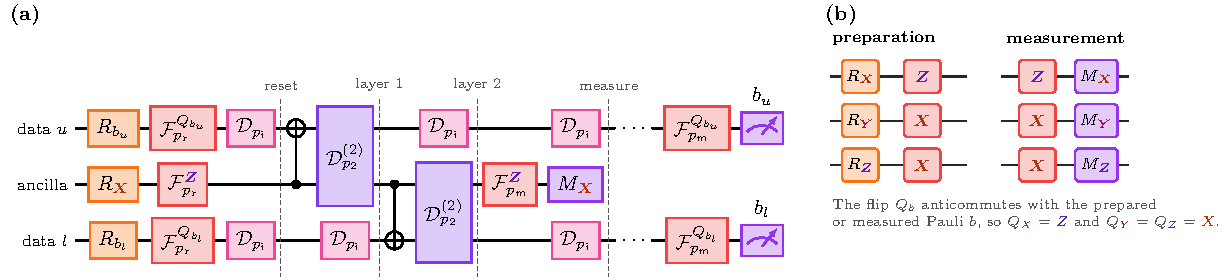
\includegraphics[width=\textwidth]{fig_noise.pdf}
  \caption{Noise channels in one round of extraction, shown for a link check $X_uX_l$. (a)~The data qubits are prepared in their frame bases $b_u$ and $b_l$ and the ancilla in $\ket{+}$, each followed by a preparation flip (red). Every layer of controlled Pauli gates is followed by a two-qubit channel on each gate pair (violet) and a single-qubit channel on every idle qubit (pink), here the depolarizing channels of SD6. The ancilla is measured in the $X$ basis after a $Z$ flip. At the end of the protocol the data qubits are read out in their frame bases after a flip. \autoref{tab:noise} lists the channels of every model. (b)~Preparation and measurement flips in the three bases, \autoref{eq:flips}. An error in an $X$-basis operation is a $Z$ error, and errors in $Y$- and $Z$-basis operations are $X$ errors.}
  \label{fig:noise}
\end{figure*}

\begin{table*}[t]
  \caption{Channels of the noise models. Each column is a location of the circuit, and each entry is the channel applied there, with the channels of \autoref{eq:dep1} to \autoref{eq:flips}. Preparation and measurement flips act in the basis $b$ of the operation. For Helios and H2 the rates are the multiples of $p$ in \autoref{eq:ionmodel}, the memory channel $\mathcal{F}^{Z}_{p_{\rm mem}}$ also acts on the qubits of every gate, and $k$ is the number of ancillas measured in the step. Under EM3 every operation is a pair measurement (MPP) or a single-qubit preparation or measurement, and $\mathcal{E}^{\rm MPP}_p$ is the error of a pair measurement defined in the text.}
  \label{tab:noise}
  \begin{ruledtabular}
  \begin{tabular}{llllll}
    Model & After each gate & Idle in gate layer & Data during reset and measurement & Preparation & Measurement \\
    \hline
    SD6 & $\mathcal{D}^{(2)}_{p}$ & $\mathcal{D}_{p}$ & $\mathcal{D}_{p}$ & $\mathcal{F}^{Q_b}_{p}$ & $\mathcal{F}^{Q_b}_{p}$ \\
    SI1000 & $\mathcal{D}^{(2)}_{p}$ & $\mathcal{D}_{p/10}$ & $\mathcal{D}_{2p}$ & $\mathcal{F}^{Q_b}_{2p}$ & $\mathcal{F}^{Q_b}_{5p}$ \\
    Biased $\eta$ & $\mathcal{N}^{(2)}_{\eta,p}$ & $\mathcal{N}_{\eta,p}$ & $\mathcal{N}_{\eta,p}$ & $\mathcal{F}^{Q_b}_{p}$ & $\mathcal{F}^{Q_b}_{p}$ \\
    Helios, H2 & $\mathcal{D}^{(2)}_{p_2}$, $\mathcal{D}_{p_1}\otimes\mathcal{D}_{p_1}$ & $\mathcal{F}^{Z}_{p_{\rm mem}}$ & $\mathcal{D}_{p^{(k)}_{\rm xt}}$, $\mathcal{F}^{Z}_{p_{\rm mem}}$ & $\mathcal{F}^{Q_b}_{p_{\rm r}}$ & $\mathcal{F}^{Q_b}_{p_{\rm m}}$ \\
    EM3 & $\mathcal{E}^{\rm MPP}_{p}$ & $\mathcal{D}_{p}$ & $\mathcal{D}_{p}$ & $\mathcal{F}^{Q_b}_{p}$ & $\mathcal{F}^{Q_b}_{p}$ \\
  \end{tabular}
  \end{ruledtabular}
\end{table*}

\subsection{Extraction with pair measurements}
\label{sec:em3}

On hardware with native pair measurements the links are single operations. Each link is measured by one pair measurement $X_uX_l$. A plaquette $P=\prod_q P_q$ of weight $w$ uses $w$ ancillas, which are prepared in $\ket{+}$ and joined into a cat state by $w-1$ pair measurements $Z_aZ_{a'}$ along a tree [\autoref{fig:em3}(a)]. Each ancilla $a_q$ is then measured jointly with its data qubit, $X_{a_q}P_q$, and read out in the $Z$ basis in the next step. Because $\prod_qX_{a_q}=+1$ on the cat state, the product of the $w$ coupling outcomes is the eigenvalue of $P$, while no smaller product of the $P_q$ is revealed, as in the cat-state extraction of Shor~\cite{shor1996}. A coupling $X_{a_q}P_q$ anticommutes with every other check $C$ that acts on $q$ with a different Pauli. After the readout, $C$ has changed sign by the $Z$ outcomes of the ancillas of $P$ on the qubits where $C$ and $P$ differ and by the parity of the cat between these ancillas, which is a product of tree outcomes. We include these signs in the detectors and in the observable. They are well defined only if two overlapping plaquettes couple to all their shared qubits in the same order. We therefore color the plaquettes with three colors, so that plaquettes of one color are disjoint, and couple them color by color. A round has four steps, one for the links and one for each color [\autoref{fig:em3}(b)]. Two banks of ancillas alternate between rounds, and the cat states of the next round are prepared while the current round couples to the data.

A wrong outcome on a tree edge has the same effect on the signs as the plaquette operator applied to the qubits below that edge. Every block of the plaquette hangs from the center of the tree, so such a fault is equivalent to an error on one qubit or on the two qubits of one block, and the same holds for an error on an ancilla. A pair measurement on a link can also apply a two-qubit error to its block. The operator $\Yb$ contains both qubits of one block, so these faults lower the circuit-level fault distance from $d+1$ to $d$. We verified $d_f=d$ exactly with CP-SAT for $d=3$ and $5$. Under EM3 the error $\mathcal{E}^{\rm MPP}_p$ of a link or cat measurement keeps the flip of the outcome correlated with the Pauli error. We simulate it with an auxiliary qubit in $\ket{0}$ that is included in the measured product as $Z$ and carries the flip. For a coupling the same distribution is a uniform two-qubit Pauli error before the measurement, because the ancilla is read out right after it.

\begin{figure*}[t]
  \centering
  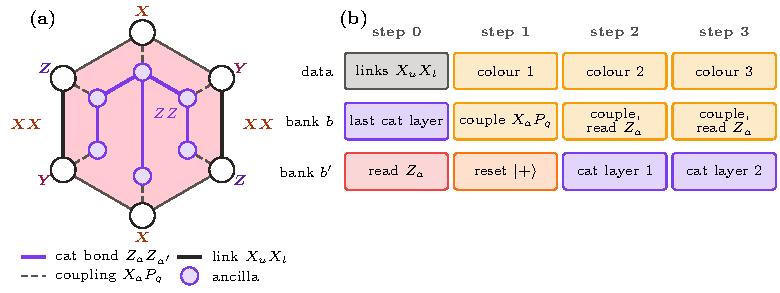
\includegraphics[width=0.92\textwidth]{fig_em3.pdf}
  \caption{Extraction with pair measurements under the EM3 model. (a)~One hexagon. The two vertical links are measured directly by $X_uX_l$. Six ancillas, one per data qubit, form a cat state through pair measurements $Z_aZ_{a'}$ along a tree (violet) whose center is the ancilla of the top qubit. Each block hangs from the center as one edge or as a path of two edges. Each ancilla is then measured jointly with its data qubit, $X_aP_q$ (dashed), where $P_q$ is the Pauli of the hexagon on that qubit (colored labels). (b)~The steps of one round. The data qubits are coupled to the plaquettes of the three colors in turn. Bank $b$ couples in this round, and bank $b'$, read out at the start of the round, prepares the cat states of the next round.}
  \label{fig:em3}
\end{figure*}

\subsection{Logical error rates below threshold}
\label{sec:scaling}

\autoref{fig:scaling} shows the logical error rate of the fault-tolerant protocol under SD6 noise. With a single round the logical error rate falls with distance over the whole range shown. At $p=10^{-3}$ we find $\pL=4.1\times10^{-4}$ and $1.9\times10^{-5}$ for $d=3$ and $5$, and about $10^{-6}$ for $d=7$. Between $p=10^{-3}$ and $2\times10^{-3}$ the rates scale as $p^{2.1}$ for $d=3$ and $p^{3.4}$ for $d=5$, close to the powers $2$ and $3$ that \autoref{eq:scaling} predicts for $d_f=d+1$. With $r=d$ rounds and MWPM the logical error rates at $p=10^{-3}$ are $1.3\times10^{-3}$, $2.5\times10^{-4}$, $4.9\times10^{-5}$ and $8\times10^{-6}$ for $d=3$ to $9$. HCM lowers them to $1.0\times10^{-3}$, $1.3\times10^{-4}$ and $1.8\times10^{-5}$ for $d=3$ to $7$.

\begin{figure}[t]
  \centering
  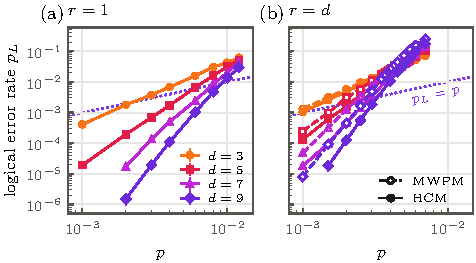
\includegraphics[width=\columnwidth]{fig_scaling.pdf}
  \caption{Logical error rate of $\plusL$ under SD6 noise. (a)~One round, decoded with MWPM. (b)~$r=d$ rounds, decoded with MWPM (dashed, open markers) and with hierarchical correlated matching (solid). The dotted line is $\pL=p$.}
  \label{fig:scaling}
\end{figure}

\subsection{Threshold and the number of rounds}
\label{sec:rounds_threshold}

The protocol can stop after any number of rounds $r$. We determined the threshold of MWPM under SD6 noise for $r=1$ to $6$, $8$ and $10$ and for $r=d$, with every odd distance from $d=3$ to $19$. The code is defined for odd $d$, so $d=19$ is the largest distance below 20. We first sampled 16 values of $p$ between $2\times10^{-3}$ and $10^{-1}$ with up to $2\times10^{4}$ shots or $200$ logical errors per point, and then eight values of $p$ around the crossing points with up to $6\times10^{4}$ shots or $1500$ logical errors. \autoref{fig:rounds_curves} shows the data around each threshold. For every $r$ the curves of the nine distances cross in a narrow window of $p$, below which the logical error rate falls with $d$. Above the window every curve rises to $\pL=1/2$, the value at which the decoder output is uncorrelated with $\Xb$, and the curves do not cross again up to $p=10^{-1}$ (Appendix~\ref{app:fits}, \autoref{fig:rounds_full}).

\begin{figure*}[t]
  \centering
  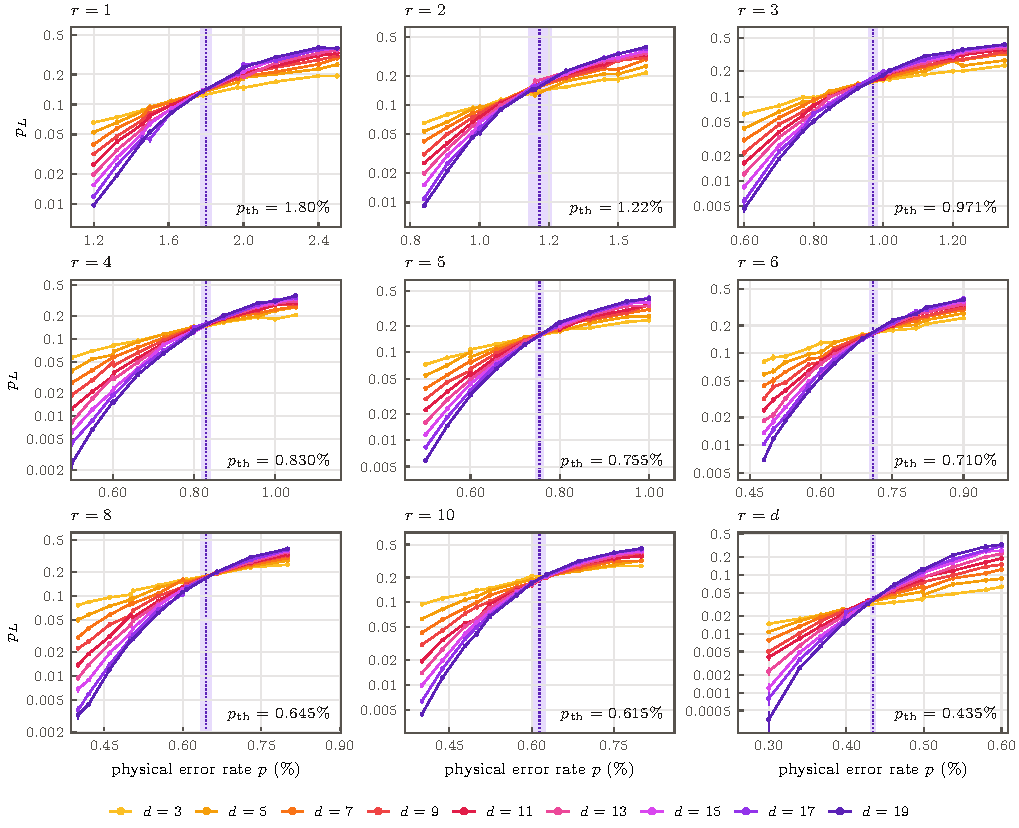
\includegraphics[width=\textwidth]{fig_rounds_curves.pdf}
  \caption{Logical error rate of $\plusL$ under SD6 noise with MWPM, for $r=1$ to $6$, $8$ and $10$ rounds and for $r=d$, with $d=3$ to $19$. Each panel shows the window $0.6\,\pth\le p\le1.4\,\pth$ around its threshold. The vertical line and band mark the threshold of \autoref{tab:rounds} and its uncertainty. \autoref{fig:rounds_full} shows the full sweep up to $p=10^{-1}$.}
  \label{fig:rounds_curves}
\end{figure*}

Near the crossing we fit the data to the finite-size scaling form
\begin{equation}
  \pL = A + Bx + Cx^2,\qquad x=(p-\pth)\,d^{1/\nu},
  \label{eq:fss}
\end{equation}
as in Ref.~\cite{wang2003}, using the distances $d=11$ to $19$. The uncertainty combines a parametric bootstrap with half the spread of fits that use other windows of $p$ and other sets of distances. \autoref{tab:rounds} and \autoref{fig:rounds_pth}(a) give the results. The threshold is $1.80(3)\%$ for one round and falls to $1.22(4)\%$ for two rounds, $0.83(1)\%$ for four and $0.61(1)\%$ for ten. For $r=d$ the crossing of the logical error rate per shot gives $0.435(3)\%$. In this family a larger code also runs more rounds, which moves the crossing down. We therefore also fit the logical error rate per round,
\begin{equation}
  \epsilon_L=\tfrac{1}{2}\Big[1-\left(1-2\pL\right)^{1/(r+1)}\Big],
  \label{eq:per_round}
\end{equation}
which treats the $r+1$ layers of $\Sz$ detectors as independent chances for a logical error. Its crossing lies at $0.501(8)\%$. A preparation that is read out or consumed after a single round therefore tolerates about four times the physical error rate at which a preparation with $r=d$ rounds fails.

\begin{table}[t]
  \caption{Threshold of MWPM as a function of the number of rounds $r$ under SD6 noise, from the fit of \autoref{eq:fss} to $d=11$ to $19$. The uncertainty combines the bootstrap error with half the spread of fits with other windows and sets of distances. For $r=d$ the fit uses either the logical error rate per shot, $\pL$, or the logical error rate per round, $\epsilon_L$ of \autoref{eq:per_round}. The last column gives the exponent $\nu$ with its bootstrap error.}
  \label{tab:rounds}
  \begin{ruledtabular}
  \begin{tabular}{lcc}
    $r$ & $p_{\mathrm{th}}$ (\%) & $\nu$ \\
    \hline
    1 & $1.800(27)$ & $1.6(3)$ \\
    2 & $1.217(42)$ & $2.2(5)$ \\
    3 & $0.971(13)$ & $1.3(1)$ \\
    4 & $0.830(12)$ & $1.3(2)$ \\
    5 & $0.755(10)$ & $1.7(2)$ \\
    6 & $0.710(9)$ & $1.7(2)$ \\
    8 & $0.645(10)$ & $1.8(2)$ \\
    10 & $0.615(11)$ & $1.9(4)$ \\
    $d$, per shot & $0.435(3)$ & $1.1(1)$ \\
    $d$, per round & $0.501(8)$ & $1.2(1)$ \\
  \end{tabular}
  \end{ruledtabular}
\end{table}

\begin{figure}[t]
  \centering
  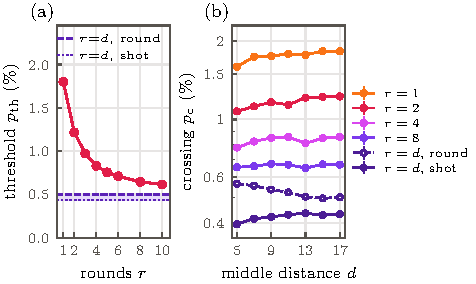
\includegraphics[width=\columnwidth]{fig_rounds_pth.pdf}
  \caption{(a)~Threshold of MWPM under SD6 noise as a function of the number of rounds. The band for $r=d$ spans the crossings of the logical error rate per shot (dotted) and per round (dashed). (b)~Crossing points $p_c$ from fits to three consecutive distances, plotted against the middle distance, with bootstrap uncertainties. For $r=d$ the open symbols use the error rate per round of \autoref{eq:per_round}.}
  \label{fig:rounds_pth}
\end{figure}

\autoref{fig:slab} explains this dependence. The $\Sz$ detectors fill a space-time box with $r+1$ layers in time. Both time boundaries are closed, because the initial state and the frame readout fix every element of $\Sz$, so an error chain can only end on the two space boundaries of the patch. A logical failure is a chain that connects these two boundaries. For fixed $r$ and growing $d$ the box becomes a thin slab, and every failing chain has to cross the full width of the patch inside it. A box of height $d+1$ contains many more chains of a given length, because they can also run diagonally in space-time. A thin slab therefore behaves like a two-dimensional matching problem whose effective error rate grows with $r$, and its threshold decreases toward that of the full space-time problem as $r$ grows.

\begin{figure}[t]
  \centering
  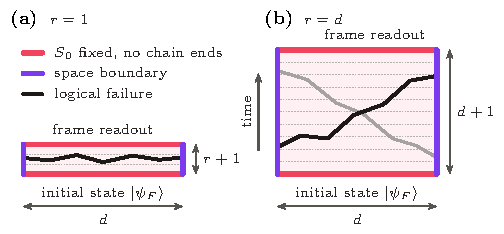
\includegraphics[width=\columnwidth]{fig_slab.pdf}
  \caption{Space-time picture of decoding on $\Sz$. The initial state and the frame readout fix every element of $\Sz$ (coral), so error chains can end only on the space boundaries of the patch (violet). A logical failure is a chain that connects the two space boundaries. (a)~With one round the chain has to cross the patch within a slab of two detector layers. (b)~With $r=d$ rounds it can also run diagonally in space-time, and there are many more such chains.}
  \label{fig:slab}
\end{figure}

The same picture explains how the crossing points move with the distance. \autoref{fig:rounds_pth}(b) shows fits of \autoref{eq:fss} to three consecutive distances. For one round the crossing rises from $1.60\%$ for $d=3$, $5$ and $7$ to $1.83\%$ for $d=15$, $17$ and $19$, as the patch becomes wide compared with the slab. For $r=d$ the crossing of the per-shot error rate rises from $0.39\%$ to $0.43\%$, and that of the per-round error rate falls from $0.57\%$ to $0.50\%$. The two estimates approach each other from opposite sides, so the threshold of the full space-time problem lies between $0.435\%$ and $0.50\%$.

For preparation, the threshold that matters is the one for the number of rounds that is actually used. Each round lowers it, because failing chains can run through more of space-time. The decrease is fast for the first few rounds and slow afterwards. With ten rounds the threshold is $0.61\%$, still about $20\%$ above the per-round threshold for $r=d$.


\subsection{Thresholds of the noise models}
\label{sec:thresholds}

We determine the thresholds of the six generic noise models and of the decoders from runs with $r=d$ rounds and $d=3$ to $9$, with points spaced by $5\%$ of the threshold around each crossing. Near the crossing point we fit the logical error rates of $d=5$, $7$ and $9$ to the finite-size scaling form of \autoref{eq:fss}. For SD6 noise and MWPM this gives $0.41\%$, slightly below the per-shot value $0.435\%$ from $d=11$ to $19$ in \autoref{sec:rounds_threshold}, so the thresholds in this section are slightly conservative. The quoted uncertainty is the larger of the statistical error of the fit and half the spread between this fit, a fit that includes $d=3$, and the crossing points of neighboring distances. \autoref{tab:thresholds} lists the results and \autoref{fig:thresholds} shows the data.

\begin{table}[t]
  \caption{Thresholds for $r=d$ rounds in percent of the physical error rate $p$. The number in parentheses is the uncertainty in the last digit. MWPM and HCM come from finite-size scaling fits with $d=5$, $7$ and $9$. BM is belief-matching, for which we quote the crossing point of $d=5$ and $d=7$ (\autoref{fig:bm}). Under EM3 the plaquettes are measured with pair measurements (\autoref{sec:em3}).}
  \label{tab:thresholds}
  \setlength{\tabcolsep}{3pt}
  \begin{ruledtabular}
  \begin{tabular}{lcccc}
    Noise model & MWPM & HCM, links & HCM & BM \\
    \hline
    SD6 & $0.41(1)$ & $0.50(1)$ & $0.50(2)$ & $0.55(2)$ \\
    SI1000 & $0.36(1)$ & $0.43(1)$ & $0.44(2)$ & $0.46(2)$ \\
    Biased, $\eta=10$ & $0.44(1)$ & $0.57(1)$ & $0.64(1)$ & $0.79(3)$ \\
    Biased, $\eta=100$ & $0.44(1)$ & $0.59(1)$ & $0.68(1)$ & $0.86(1)$ \\
    Pure $Z$ & $0.44(1)$ &  & $0.69(1)$ & $0.83(4)$ \\
    EM3 & $0.22(1)$ &  & $0.28(1)$ &  \\
  \end{tabular}
  \end{ruledtabular}
\end{table}

\begin{figure*}[t]
  \centering
  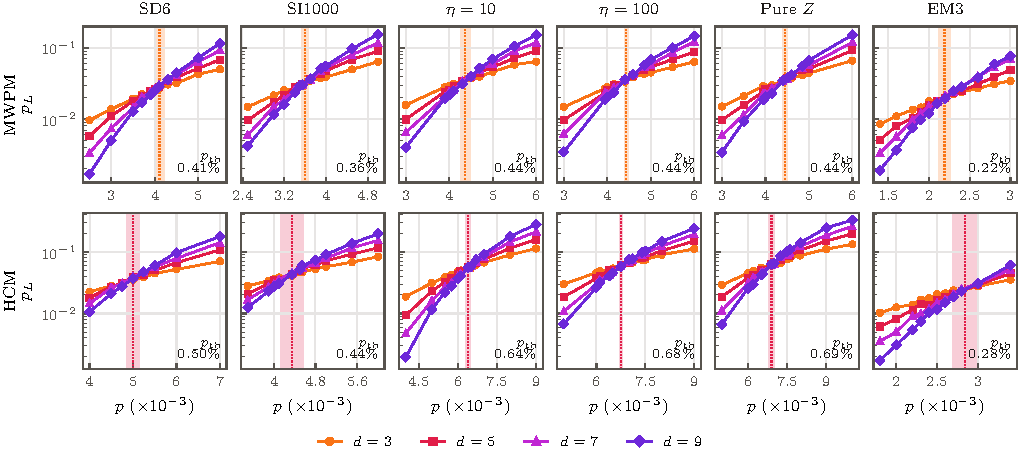
\includegraphics[width=\textwidth]{fig_thresholds.pdf}
  \caption{Threshold crossings for $r=d$ rounds and $d=3$ to $9$. Top row, matching on the $\Sz$ detectors. Bottom row, hierarchical correlated matching. Vertical lines and bands mark the fitted threshold and its uncertainty.}
  \label{fig:thresholds}
\end{figure*}

Matching on $\Sz$ reaches thresholds between $0.36\%$ for SI1000 and $0.44\%$ for biased noise, and $0.22\%$ under EM3. Hierarchical correlated matching raises every threshold. The gain is $22\%$ for SD6, $21\%$ for SI1000 and $30\%$ for EM3, and it grows with the bias, to $46\%$ for $\eta=10$, $53\%$ for $\eta=100$ and $55\%$ for pure $Z$ noise.

The lower level is responsible for the gain. Under $Z$-biased noise most faults are $Z$ errors on data qubits. Apart from $Z$ errors on the upper vertex of an odd block, which leave every element of $\Sz$ unchanged, such an error flips $\Sz$ detectors and at the same time an odd link or a class-A hexagon. The lower level therefore marks most of the upper edges that the faults have flipped, and the second matching pass follows these marks. Matching on $\Sz$ alone cannot use this structure, and its threshold hardly changes with the bias, from $0.41\%$ for SD6 to $0.44\%$ for $\eta=10$, $\eta=100$ and pure $Z$ noise. The tolerance of the code to biased noise is available only to a decoder that reads the gauge level. The odd links alone account for the full gain under SD6 and SI1000 noise. Under biased noise the class-A hexagons add a further $12\%$ to $15\%$ to the threshold. Among the decoders of \autoref{tab:thresholds}, belief-matching, which we ran up to $d=7$, gives the highest thresholds. Its threshold is $0.55\%$ for SD6, $0.79\%$ for $\eta=10$, $0.86\%$ for $\eta=100$ and $0.83\%$ for pure $Z$ noise, close to twice the threshold of matching under strong bias (\autoref{tab:thresholds} and Appendix~\ref{app:fits}). Under SI1000 noise, in which measurement errors dominate, belief-matching and HCM reach nearly the same threshold.

Under EM3 the thresholds are about half of those for SD6, $0.22\%$ for matching and $0.28\%$ for HCM. A weight-six plaquette takes eleven noisy pair measurements and six readouts, and its ancillas idle until the step of their color, so every plaquette outcome carries several times the error of a single operation. The honeycomb code, whose checks are the pair measurements themselves, reaches $1.5\%$ to $2\%$ under the same model~\cite{gidney2021honeycomb}. A schedule in which the plaquettes of the $XYZ^2$ code are inferred from link measurements in the same way is a natural alternative for such hardware, which we leave for future work.

\subsection{Decoder comparison}
\label{sec:decoder_comparison}

\autoref{fig:decoders} compares the decoders at $d=3$ and $d=5$ with $r=d$ rounds. Under SD6 noise at $d=5$ and $p=4\times10^{-3}$, erasure passing raises the logical error rate of matching by $62\%$. Sequential BP lowers it by $21\%$, both versions of HCM by $32\%$ and belief-matching by about $40\%$. Tesseract, our near-optimal reference, reaches $1.3(2)\times10^{-2}$, about $20\%$ below belief-matching. At $d=3$ belief-matching is within about $15\%$ of Tesseract.

Erasure passing fails because a matched link edge marks every fault with that link signature, and the $\Sz$ edges of all of these faults are erased. Most of the marked faults did not occur, and the erased edges open short paths for the upper matching. Sequential BP passes the same information as probabilities and avoids this problem. Its gain is limited because the link detectors see only part of each fault.

Under biased noise the differences grow. At $d=5$, $p=5\times10^{-3}$ and $\eta=100$, sequential BP lowers the logical error rate of matching by a factor of $1.8$, HCM with links by $2.0$, HCM by $2.9$ and belief-matching by $5.3$. Tesseract reaches $4.5(10)\times10^{-3}$ at this point, about half the rate of belief-matching, so a decoder closer to the optimum still has room to gain under bias. \autoref{sec:cfe_results} shows that the coset free-energy decoder closes this gap. In this regime the class-A hexagons carry as much information as the links, and BP on the full detector error model uses it most completely. Belief-matching is, however, about 240 times slower than HCM in our implementation, because BP runs over the full DEM for every shot (\autoref{tab:decoders}). HCM obtains a large part of the gain at about four times the cost of matching.

\begin{figure*}[t]
  \centering
  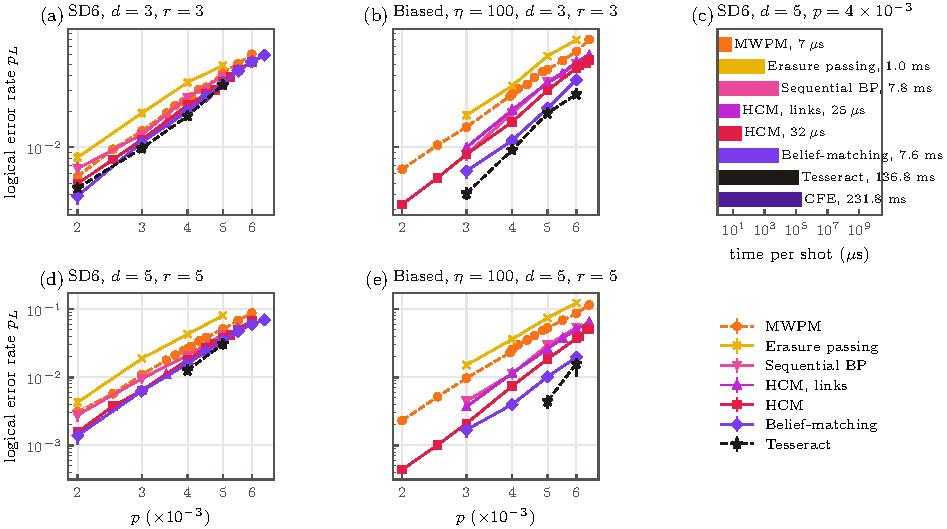
\includegraphics[width=\textwidth]{fig_decoders.pdf}
  \caption{Comparison of decoders with $r=d$ rounds. (a,b)~$d=3$ under SD6 noise and under biased noise with $\eta=100$. (d,e)~The same for $d=5$. Dashed lines are matching on $\Sz$ and Tesseract, and points with fewer than eight logical errors are not shown. (c)~Decoding time per shot at $d=5$ and $p=4\times10^{-3}$ under SD6 noise on one core.}
  \label{fig:decoders}
\end{figure*}


\subsection{Coset free-energy decoding}
\label{sec:cfe_results}

\autoref{tab:cfe} separates the steps of the CFE decoder at $d=5$ with five rounds, on the same 3000 shots for every decoder. Under biased noise with $\eta=100$ and $p=5\times10^{-3}$, BP-OSD fails on 25 shots and the two-class search on 23. The local descent lowers this to 14, the free energy to 13 and the guided candidates to 12. Tesseract fails on 15 of the same shots and belief-matching on 30. Under SD6 noise at the same $p$, the two-class search alone fails on 146 shots, more than BP-OSD with a single class (117) and belief-matching (102), because BP-OSD often returns a heavy error in one of the two classes. The descent removes most of this excess, and the free energy and the guided candidates bring the CFE decoder to 84 failures, the same as Tesseract (85) and $18\%$ below belief-matching. The free energy changes the decision mostly in shots where the two candidates have similar weight, and its effect is largest under SD6 noise, where $Y$ errors and their $X$ and $Z$ parts give many equivalent errors. The results depend little on $\kappa$. Any value between $0.2$ and $0.8$ gives between 82 and 91 failures under SD6 noise and 12 under biased noise.

\begin{table}[t]
  \caption{Logical failures of the decoders on the same 3000 shots at $d=5$, $r=5$ and $p=5\times10^{-3}$. The middle rows add the steps of the CFE decoder one at a time.}
  \label{tab:cfe}
  \begin{ruledtabular}
  \begin{tabular}{lcc}
    Decoder & SD6 & Biased, $\eta=100$ \\
    \hline
    MWPM & 187 & 162 \\
    HCM & 109 & 58 \\
    Belief-matching & 102 & 30 \\
    BP-OSD & 117 & 25 \\
    Two-class BP-OSD & 146 & 23 \\
    \quad + local descent & 108 & 14 \\
    \quad + free energy, $\kappa=1/2$ & 103 & 13 \\
    \quad + guided candidates (CFE) & 84 & 12 \\
    Tesseract & 85 & 15 \\
  \end{tabular}
  \end{ruledtabular}
\end{table}

\autoref{fig:cfe_thr} and \autoref{tab:cfe_thr} follow the comparison with belief-matching to larger distances, again on the same shots, for $r=d$ rounds and $d=3$, $5$ and $7$. Under biased noise with $\eta=100$ the CFE decoder fails on $11\%$, $21\%$ and $28\%$ fewer shots than belief-matching at $d=3$, $5$ and $7$. Its advantage grows with the distance, which points to a higher threshold under strong bias, although the $d=7$ points, with 600 shots each, do not resolve the crossing well enough to quote one. Under SD6 noise the CFE decoder is $4\%$ and $6\%$ better at $d=3$ and $5$, but at $d=7$ it fails on $18(12)\%$ more shots than belief-matching. The two-class search is the weak point at larger distances. BP-OSD returns heavier errors as the detector error model grows, and moves of three or four faults cannot repair a candidate that differs from the best error along a long chain. A third pair of candidates, guided by the solution of belief-matching in the same way as the HCM guide, lowers the failures at $d=7$ from 120 to 111, against 102 for belief-matching. Under depolarizing noise the decoder therefore needs a candidate search that scales with the code. The cost is about $2$~s per shot at $d=7$ in our Python implementation, against $0.3$~s at $d=5$.

\begin{figure*}[t]
  \centering
  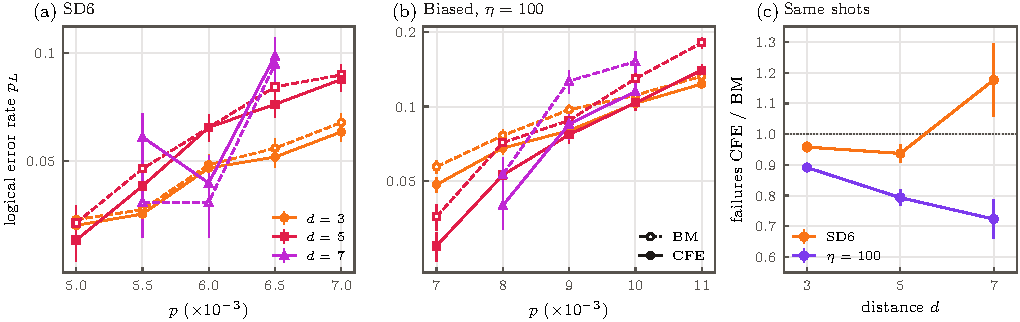
\includegraphics[width=\textwidth]{fig_cfe_thr.pdf}
  \caption{CFE decoding against belief-matching on the same shots with $r=d$ rounds. (a)~SD6 and (b)~biased noise with $\eta=100$, decoded with CFE (solid, filled markers) and belief-matching (BM, dashed, open markers). The points for $d=7$ use 600 shots each, those for $d=5$ and $d=3$ use 2000 and 4000. (c)~Failures of CFE divided by failures of belief-matching, summed over $p$, as a function of the distance.}
  \label{fig:cfe_thr}
\end{figure*}

\begin{table}[t]
  \caption{Failures of the CFE decoder and of belief-matching on the same shots with $r=d$, summed over the values of $p$ in \autoref{fig:cfe_thr}. The last column is their ratio with its bootstrap error.}
  \label{tab:cfe_thr}
  \begin{ruledtabular}
  \begin{tabular}{llrrrc}
    Noise & $d$ & Shots & CFE & BM & CFE/BM \\
    \hline
    SD6 & 3 & 20000 & 911 & 951 & $0.96(2)$ \\
     & 5 & 10000 & 582 & 621 & $0.94(3)$ \\
     & 7 & 1800 & 120 & 102 & $1.18(12)$ \\
    $\eta=100$ & 3 & 20000 & 1691 & 1897 & $0.89(2)$ \\
     & 5 & 10000 & 802 & 1011 & $0.79(3)$ \\
     & 7 & 1800 & 144 & 199 & $0.72(6)$ \\
  \end{tabular}
  \end{ruledtabular}
\end{table}

\section{Implementation on Quantinuum hardware}
\label{sec:hardware}

\subsection{Circuits and resources}

Quantinuum processors have all-to-all connectivity, mid-circuit measurement and reset, and conditional operations~\cite{moses2023,ransford2026}. The interleaved schedule of \autoref{sec:schedule} therefore needs no routing. Helios stores 98 $^{137}$Ba$^+$ ions and implements the native gates
\begin{align}
  R_{ZZ}(\theta)&=e^{-i\theta Z\otimes Z/2},\nonumber\\
  U_{1q}(\theta,\phi)&=e^{-i\theta(\cos\phi\,X+\sin\phi\,Y)/2},
  \label{eq:native}
\end{align}
together with $R_Z(\theta)=e^{-i\theta Z/2}$, which is applied in software and has no error~\cite{ransford2026}. Every controlled Pauli of the extraction circuit compiles to one native two-qubit gate,
\begin{align}
  \mathrm{C}Z&=e^{i\pi/4}\,\big[R_Z(\tfrac{\pi}{2})\otimes R_Z(\tfrac{\pi}{2})\big]\,R_{ZZ}(-\tfrac{\pi}{2}),\nonumber\\
  \mathrm{C}P&=(I\otimes V_P)\,\mathrm{C}Z\,(I\otimes V_P^\dagger),
  \label{eq:compile}
\end{align}
where the ancilla is the first qubit and $V_P$ is a single-qubit Clifford with $V_PZV_P^\dagger=P$, for example $V_X=H$. $V_P$ costs one $U_{1q}$ gate on the data qubit, up to software $R_Z$ rotations. \autoref{tab:resources} lists the resources per round.

The $d=3$ protocol uses 18 data qubits and 17 ancillas, 35 qubits in total, and 54 two-qubit gates per round. It fits on H2 and on Helios. The $d=5$ protocol needs 50 data qubits and 49 ancillas, one more than the 98 qubits of Helios. The link ancillas finish after the second layer, while some boundary checks start in the third layer or later. We measure and reset four link ancillas after the second layer and reuse them for four boundary checks. This brings $d=5$ to 95 qubits with 170 two-qubit gates per round. The reuse adds one mid-circuit measurement step per round. In our simulations it changes neither the fault distance nor, within the statistical error, the logical error rate.

The circuits are exported as OpenQASM~2.0 together with the annotated Stim circuit, which defines the detectors and the observable. The measurement record of each hardware shot is decoded with the same detector error model as in the simulations. Preparation and verification do not require real-time decoding, because the decoder only has to correct the final readout. When the state is used in a computation, the logical bit enters the Pauli frame. Matching takes about $7\,\mu$s and HCM about $30\,\mu$s per shot at $d=5$, which is short compared with the duration of an extraction round on trapped ions.

\begin{table}[t]
  \caption{Resources per extraction round. Two-qubit gates are native $ZZ$ gates. For $d=5$ on Helios, four ancillas are reused within each round.}
  \label{tab:resources}
  \begin{ruledtabular}
  \begin{tabular}{lcccc}
    & Data & Ancillas & Total & 2Q gates \\
    \hline
    $d=3$ & 18 & 17 & 35 & 54 \\
    $d=5$ & 50 & 49 & 99 & 170 \\
    $d=5$, reuse & 50 & 45 & 95 & 170 \\
    $d=7$ & 98 & 97 & 195 & 350 \\
  \end{tabular}
  \end{ruledtabular}
\end{table}

\subsection{The Helios noise model}
\label{sec:helios_model}

The Helios data sheet quotes five typical error rates, averaged over all operation zones~\cite{helios_datasheet}, and Ref.~\cite{ransford2026} measures each of them independently. We convert them into Pauli channels as follows. Randomized benchmarking quotes an average infidelity $\epsilon$. A depolarizing channel on $n$ qubits with total Pauli error probability $p$ has
\begin{equation}
  \epsilon=\frac{2^n}{2^n+1}\,p,
  \label{eq:infidelity}
\end{equation}
and a single Pauli flip with probability $p$ has $\epsilon=2p/3$. The Helios model consists of the following channels:
\begin{enumerate}
  \item \emph{Gates.} Every controlled Pauli is followed by $\mathcal{D}^{(2)}_{p_2}$ with $p_2=\tfrac{5}{4}\epsilon_2$ and by $\mathcal{D}_{p_1}$ on both qubits with $p_1=\tfrac{3}{2}\epsilon_1$, which accounts for the $U_{1q}$ gates of \autoref{eq:compile}.
  \item \emph{Memory.} The data sheet quotes the memory error per qubit during an average depth-1 circuit, a layer in which every qubit takes part in at most one two-qubit gate. This error is dephasing from the transport and idle periods~\cite{ransford2026}. We apply $\mathcal{F}^{Z}_{p_{\rm mem}}$ with $p_{\rm mem}=\tfrac{3}{2}\epsilon_{\rm mem}$ to every qubit in every gate layer and to the data qubits in every measurement step.
  \item \emph{Measurement crosstalk.} Scattered light from the measurement or reset of one ion can project or depolarize the other ions in the trap. The data sheet quotes this error as a global average over the trap~\cite{helios_datasheet}, with infidelity $\epsilon_{\rm xt}$ per spectator qubit and per measured qubit~\cite{ransford2026}. A step that measures and resets $k$ ancillas therefore applies $k$ such events to every data qubit, which compose to
  \begin{equation}
    \mathcal{D}_{p_{\rm xt}^{(k)}},\qquad p_{\rm xt}^{(k)}=\tfrac{3}{4}\Big[1-\big(1-\tfrac{4}{3}p_{\rm xt}\big)^{k}\Big],\qquad p_{\rm xt}=\tfrac{3}{2}\epsilon_{\rm xt}.
    \label{eq:xtalk}
  \end{equation}
  \item \emph{Preparation and measurement.} The SPAM error $\epsilon_{\rm SPAM}$ is the probability of a wrong outcome and is split evenly into the flips $p_{\rm r}=p_{\rm m}=\epsilon_{\rm SPAM}/2$ of \autoref{eq:flips}.
\end{enumerate}
The H2 model uses the same channels with the rates of the H2 data sheet~\cite{h2_datasheet}. \autoref{tab:noise} summarizes the channels and \autoref{tab:qparams} the rates.

We use the data sheets only to fix the ratios between the rates, in the same way as the SI1000 model fixes the ratios of a superconducting device~\cite{gidney2021honeycomb}. The single parameter is the two-qubit depolarizing probability $p=p_2$, and every other rate keeps its ratio to $p$ from \autoref{tab:qparams},
\begin{align}
  \text{Helios:}\quad &p_1=0.045\,p,\quad p_{\rm r}=p_{\rm m}=0.25\,p,\nonumber\\
  &p_{\rm mem}=0.9\,p,\quad p_{\rm xt}=0.075\,p,\nonumber\\
  \text{H2:}\quad &p_1=0.024\,p,\quad p_{\rm r}=p_{\rm m}=0.4\,p,\nonumber\\
  &p_{\rm mem}=0.4\,p,\quad p_{\rm xt}=0.008\,p.
  \label{eq:ionmodel}
\end{align}
The devices of the data sheets sit at $p_0=1.0\times10^{-3}$ for Helios and $p_0=1.9\times10^{-3}$ for H2. A value $p<p_0$ describes a device with the same error budget and smaller errors. The data sheet quotes maximum rates between $1.7$ and $14$ times the typical ones~\cite{helios_datasheet}, so the range $p\le3p_0$ of our scans covers the spread between operation zones and between days.

We checked the model against two independent sources. First, every data-sheet rate agrees with its dedicated measurement on Helios~\cite{ransford2026} within the stated uncertainty or within $25\%$, and where they differ the data sheet is the more pessimistic value. Second, the noise model of Quantinuum's own Helios emulator~\cite{quantinuum_emulator} has the same structure. It applies faults after one- and two-qubit gates with probabilities $2.5\times10^{-5}$ and $8\times10^{-4}$, partly as spontaneous emission and partly as asymmetric depolarizing noise, dephasing that grows with the duration of transport and idling, and a crosstalk fault on every other qubit in the trap at each mid-circuit measurement and reset, with probability $5.5\times10^{-5}$ per measurement and $3.5\times10^{-6}$ per reset. The emulator therefore also scales the crosstalk on a data qubit with the number of measured ancillas. Our rates are between one and two times those of the emulator, because we convert infidelities into Pauli probabilities with \autoref{eq:infidelity}, whereas the emulator uses the infidelities as fault probabilities. The model omits the following effects. Leakage, $2.4(1)\times10^{-4}$ per two-qubit gate~\cite{ransford2026}, enters only through the gate infidelity. The readout error is asymmetric, with $p(1|0)=8.1\times10^{-4}$ and $p(0|1)=1.6\times10^{-4}$, and we use its average. The three ions next to a measured ion see a larger crosstalk of $2.1(1)\times10^{-4}$, which is part of the global average. Finally, we apply the full memory error of a depth-1 circuit on 98 qubits to every layer, although our layers contain fewer gates. These choices make the model slightly pessimistic.

The rates translate into the following error per data qubit and round. At $d=5$ a data qubit takes part in $3.4$ controlled Pauli gates on average, which gives an error probability of about $2.9\times10^{-3}$. It sees seven memory steps, a $Z$ flip probability of $6.3\times10^{-3}$, and the crosstalk of $k=49$ measured ancillas, $p_{\rm xt}^{(49)}=3.7\times10^{-3}$ from \autoref{eq:xtalk}. The crosstalk grows linearly with the number of ancillas and hence with $d^2$, from $1.3\times10^{-3}$ at $d=3$ to $1.2\times10^{-2}$ at $d=9$, while the other contributions do not depend on $d$.

\begin{table*}[t]
  \caption{Error rates of the Quantinuum models and of the published data they are built from. The data-sheet values are typical average infidelities averaged over all operation zones, except the SPAM error, which is the probability of a wrong outcome. The measured Helios values come from randomized benchmarking and from dedicated SPAM, memory and crosstalk experiments~\cite{ransford2026}. The emulator values are fault probabilities of Quantinuum's emulators~\cite{quantinuum_emulator}. The model parameters follow from the conversions of \autoref{sec:helios_model} and are the values at the device point $p=p_0$ of \autoref{eq:ionmodel}.}
  \label{tab:qparams}
  \begin{ruledtabular}
  \setlength{\tabcolsep}{5pt}
  \begin{tabular}{lllll}
    Error & Data sheet & Measured & Emulator & Model \\
    \hline
    \multicolumn{5}{l}{\emph{Helios}, data sheet version 1.2~\cite{helios_datasheet}} \\
    Single-qubit gate & $\epsilon_1=3\times10^{-5}$ & $2.5(1)\times10^{-5}$ & $2.5\times10^{-5}$ & $p_1=4.5\times10^{-5}$ \\
    Two-qubit gate & $\epsilon_2=8\times10^{-4}$ & $7.9(2)\times10^{-4}$ & $8\times10^{-4}$ & $p_2=1.0\times10^{-3}$ \\
    SPAM & $\epsilon_{\rm SPAM}=5\times10^{-4}$ & $4.8(6)\times10^{-4}$ & $5\times10^{-4}$, reset & $p_{\rm r}=p_{\rm m}=2.5\times10^{-4}$ \\
    Memory, depth-1 circuit & $\epsilon_{\rm mem}=6\times10^{-4}$ & $5(1)\times10^{-4}$ & dephasing & $p_{\rm mem}=9\times10^{-4}$ \\
    Crosstalk per ancilla & $\epsilon_{\rm xt}=5\times10^{-5}$ & $4.8(1)\times10^{-5}$ & $5.9\times10^{-5}$ & $p_{\rm xt}=7.5\times10^{-5}$ \\
    \hline
    \multicolumn{5}{l}{\emph{H2}, data sheet version 2.00~\cite{h2_datasheet}} \\
    Single-qubit gate & $\epsilon_1=3\times10^{-5}$ &  & $1.9\times10^{-5}$ & $p_1=4.5\times10^{-5}$ \\
    Two-qubit gate & $\epsilon_2=1.5\times10^{-3}$ &  & $1.05\times10^{-3}$ & $p_2=1.9\times10^{-3}$ \\
    SPAM & $\epsilon_{\rm SPAM}=1.5\times10^{-3}$ &  & $1.0\times10^{-3}$, readout & $p_{\rm r}=p_{\rm m}=7.5\times10^{-4}$ \\
    Memory, depth-1 circuit & $\epsilon_{\rm mem}=5\times10^{-4}$ &  & dephasing & $p_{\rm mem}=7.5\times10^{-4}$ \\
    Crosstalk per ancilla & $\epsilon_{\rm xt}=1\times10^{-5}$ &  & $6.6\times10^{-6}$ & $p_{\rm xt}=1.5\times10^{-5}$ \\
  \end{tabular}
  \end{ruledtabular}
\end{table*}

\subsection{Projected performance}

\autoref{fig:quantinuum} and \autoref{tab:quantinuum} show the logical error rates. With one round and the data-sheet rates, HCM prepares $\plusL$ with $\pL=8.5\times10^{-4}$ at $d=3$ and $8.4\times10^{-5}$ at $d=5$, and the projection for $d=7$ is $1.4\times10^{-5}$. The $d=3$ value lies above the physical SPAM error of $5\times10^{-4}$, so a distance-3 preparation does not yet beat the preparation and measurement of a physical qubit. The $d=5$ value is six times below the SPAM error and ten times below the two-qubit infidelity, with 95 of the 98 qubits. With one round there are no gauge detectors, since a gauge outcome becomes a detector only in comparison with a previous round, so HCM reduces to correlated matching on $\Sz$ and agrees with MWPM within $50\%$.

With $r=d$ rounds HCM gives $1.8\times10^{-3}$, $6.7\times10^{-4}$ and $4.2\times10^{-4}$ for $d=3$, $5$ and $7$, two to four times less than MWPM, but $d=9$ is no better than $d=7$ at $p=p_0$ [\autoref{fig:quantinuum}(b)]. At $p=p_0/2$ HCM still lowers the rate by a factor of five to seven per step in distance up to $d=7$. The curves of consecutive distances do not cross at one point. With MWPM the curves of $d=3$ and $5$ cross at $p=1.54(8)\times10^{-3}$, those of $d=5$ and $7$ at $1.10(2)\times10^{-3}$ and those of $d=7$ and $9$ at $0.81(2)\times10^{-3}$, below the operating point [\autoref{fig:quantinuum}(f)]. HCM moves the last two crossings to $1.38(2)\times10^{-3}$ and $0.95(5)\times10^{-3}$. The reason is the crosstalk of \autoref{eq:xtalk}, whose contribution per data qubit and round grows with $d^2$, so a threshold in $p$ does not exist for this model. Without the crosstalk the crossings stop moving, and the Helios model has a threshold of about $2.8\times10^{-3}$, almost three times its operating point. Larger codes on a device of this kind need less crosstalk per measured ion, or measurements that shield the spectators. The H2 model shows the effect. Its crosstalk per measured ancilla is five times smaller, its crossings drift only from $3.7\times10^{-3}$ to $3.3\times10^{-3}$, about twice its operating point, and its logical error rate keeps falling, to $1.7\times10^{-4}$ at $d=7$.

The logical error rate grows linearly with the number of rounds [\autoref{fig:quantinuum}(c)]. A weighted linear fit from $r=1$ to $7$ gives an error per additional round of $4.8\times10^{-4}$, $1.4\times10^{-4}$ and $6.9\times10^{-5}$ for $d=3$, $5$ and $7$ with HCM, and $1.2\times10^{-3}$, $4.0\times10^{-4}$ and $2.1\times10^{-4}$ with MWPM. The intercepts agree with the one-round values, which are smaller than the error per additional round for the reason shown in \autoref{fig:slab}. For preparation alone a single round is the best choice.

\autoref{tab:budget} shows which errors limit these numbers. At $d=3$ and $d=5$, removing the memory error lowers the logical error rate by a factor of six to ten, removing the gate errors by a factor of two to four, and removing the crosstalk by a factor of three to four at $d=5$ but only $1.2$ to $1.3$ at $d=3$. At $d=7$ with seven rounds the crosstalk becomes the largest contribution, and removing it lowers the logical error rate by a factor of 15. SPAM errors contribute $10\%$ to $15\%$. If the crosstalk acted once per reset step and once per measurement step instead of once per measured ancilla, as it would if all ancillas shared one pulse, the rate at $d=5$ would fall by a factor of three to four. For the circuits that fit on Helios, dephasing during transport and idling is thus the main target, and for larger codes the crosstalk. With the two-qubit error rates measured by cycle benchmarking~\cite{ransford2026}, which are dominated by $Z$-type errors, the logical error rates are up to $30\%$ lower than with depolarizing gate noise (\autoref{tab:quantinuum}).

\begin{table*}[t]
  \caption{Error budget of the Helios model at the device point $p=p_0$, decoded with HCM. Each row removes one component of the model. The last row applies the crosstalk once per reset step and once per measurement step instead of once per measured ancilla.}
  \label{tab:budget}
  \begin{ruledtabular}
  \begin{tabular}{lccccc}
    & \multicolumn{2}{c}{$r=1$} & \multicolumn{3}{c}{$r=d$} \\
    \cmidrule(lr){2-3}\cmidrule(lr){4-6}
    & $d=3$ & $d=5$ & $d=3$ & $d=5$ & $d=7$ \\
    \hline
    Full model & $8.3\times10^{-4}$ & $9.1\times10^{-5}$ & $1.6\times10^{-3}$ & $7.0\times10^{-4}$ & $4.6\times10^{-4}$ \\
    No gate errors & $4.7\times10^{-4}$ & $3.4\times10^{-5}$ & $7.1\times10^{-4}$ & $1.6\times10^{-4}$ & $8.1\times10^{-5}$ \\
    No memory errors & $9.5\times10^{-5}$ & $9.2\times10^{-6}$ & $2.8\times10^{-4}$ & $8.1\times10^{-5}$ & $4.8\times10^{-5}$ \\
    No crosstalk & $6.3\times10^{-4}$ & $2.9\times10^{-5}$ & $1.3\times10^{-3}$ & $1.9\times10^{-4}$ & $3.1\times10^{-5}$ \\
    No SPAM errors & $7.0\times10^{-4}$ & $7.9\times10^{-5}$ & $1.5\times10^{-3}$ & $6.5\times10^{-4}$ & $4.1\times10^{-4}$ \\
    Crosstalk per step & $5.4\times10^{-4}$ & $3.3\times10^{-5}$ & $1.4\times10^{-3}$ & $1.9\times10^{-4}$ & $3.0\times10^{-5}$ \\
  \end{tabular}
  \end{ruledtabular}
\end{table*}

\begin{figure*}[t]
  \centering
  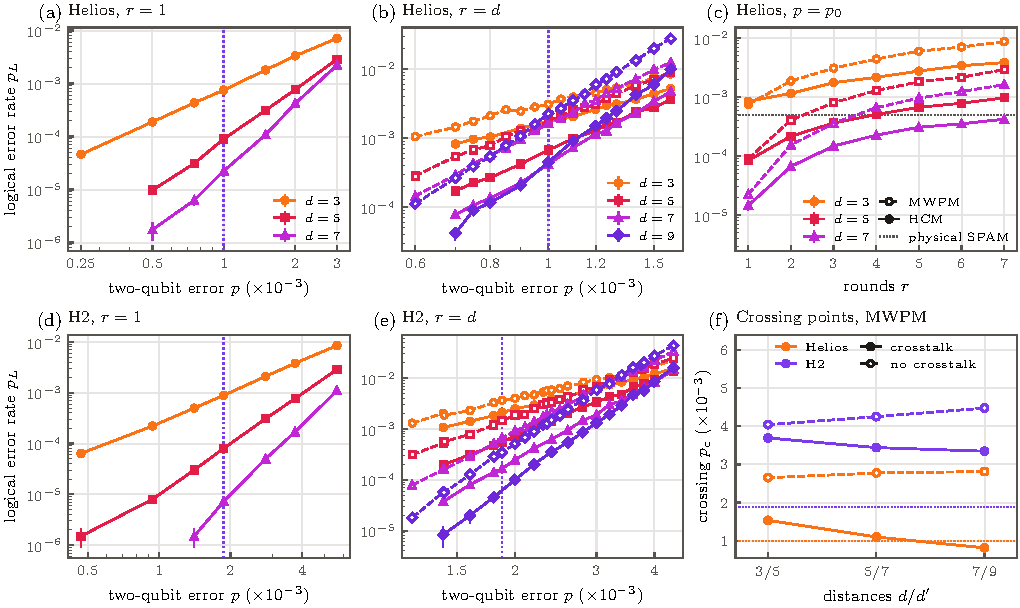
\includegraphics[width=\textwidth]{fig_quantinuum.pdf}
  \caption{Logical error rate of $\plusL$ under the one-parameter Helios and H2 models of \autoref{eq:ionmodel} as a function of the two-qubit error rate $p$. The vertical dotted lines mark the operating points $p_0$ of the data sheets. (a,d)~One round, decoded with MWPM. The curves do not cross up to $p=3p_0$. (b,e)~$r=d$ rounds around the crossing points, decoded with MWPM (dashed, open markers) and HCM (solid). (c)~Logical error rate as a function of the number of rounds at $p=p_0$ for Helios. The horizontal dotted line is the physical SPAM error. (f)~Crossing points of consecutive distances for $r=d$ and MWPM, with and without the measurement crosstalk. The horizontal lines mark $p_0$. Helios holds the circuits up to $d=5$ and H2 up to $d=3$, and larger distances are projections for larger devices with the same rates.}
  \label{fig:quantinuum}
\end{figure*}

\begin{table*}[t]
  \caption{Logical error rate of $\plusL$ under the Quantinuum models at the device point $p=p_0$. Helios, CB uses the two-qubit Pauli error rates measured by cycle benchmarking~\cite{ransford2026} instead of depolarizing gate noise. The physical SPAM error is $5\times10^{-4}$ for Helios and $1.5\times10^{-3}$ for H2. Helios holds the protocol up to $d=5$ and H2 up to $d=3$.}
  \label{tab:quantinuum}
  \setlength{\tabcolsep}{4pt}
  \begin{ruledtabular}
  \begin{tabular}{llcccccc}
    & & \multicolumn{3}{c}{$r=1$} & \multicolumn{3}{c}{$r=d$} \\
    \cmidrule(lr){3-5}\cmidrule(lr){6-8}
    Model & Decoder & $d=3$ & $d=5$ & $d=7$ & $d=3$ & $d=5$ & $d=7$ \\
    \hline
    Helios & HCM & $8.5\times10^{-4}$ & $8.4\times10^{-5}$ & $1.4\times10^{-5}$ & $1.8\times10^{-3}$ & $6.7\times10^{-4}$ & $4.2\times10^{-4}$ \\
     & MWPM & $7.5\times10^{-4}$ & $9.0\times10^{-5}$ & $2.2\times10^{-5}$ & $3.1\times10^{-3}$ & $1.8\times10^{-3}$ & $1.6\times10^{-3}$ \\
    Helios, CB & HCM & $6.5\times10^{-4}$ & $6.3\times10^{-5}$ & $1.3\times10^{-5}$ & $1.3\times10^{-3}$ & $4.6\times10^{-4}$ & $3.0\times10^{-4}$ \\
     & MWPM & $6.3\times10^{-4}$ & $7.4\times10^{-5}$ & $1.6\times10^{-5}$ & $2.7\times10^{-3}$ & $1.4\times10^{-3}$ & $1.2\times10^{-3}$ \\
    H2 & HCM & $8.9\times10^{-4}$ & $8.7\times10^{-5}$ & $8.0\times10^{-6}$ & $2.1\times10^{-3}$ & $5.5\times10^{-4}$ & $1.7\times10^{-4}$ \\
     & MWPM & $8.9\times10^{-4}$ & $8.1\times10^{-5}$ & $7.2\times10^{-6}$ & $3.7\times10^{-3}$ & $1.5\times10^{-3}$ & $6.6\times10^{-4}$ \\
  \end{tabular}
  \end{ruledtabular}
\end{table*}

\subsection{Proposed experiment}

We propose the following experiment on Helios:
\begin{enumerate}
  \item Prepare $\plusL$ with $d=3$ and with $d=5$ using $r=1,2,3$ rounds, and read out in the frame basis.
  \item Decode every shot with the detector error model of the circuit and record the corrected value of $\Xb$.
  \item Fit the logical error rate as a linear function of $r$. The slope is the logical error per round and the intercept is the error of preparation and readout.
\end{enumerate}
The model predicts $\pL=8.5\times10^{-4}$, $1.2\times10^{-3}$ and $1.8\times10^{-3}$ for $d=3$ and $r=1$, $2$ and $3$, and $8.4\times10^{-5}$, $2.2\times10^{-4}$ and $3.6\times10^{-4}$ for $d=5$. Measuring $8\times10^{-5}$ with a relative uncertainty of $20\%$ takes about $3\times10^{5}$ shots, and the $d=3$ values need ten times fewer. The slope tests the error per round, which in our model is dominated by memory and crosstalk, and the intercept tests the preparation itself. The $d=3$ experiment fits on H2 as well, where the model predicts $8.9\times10^{-4}$ for one round, below the H2 SPAM error of $1.5\times10^{-3}$.

\section{Conclusion}
\label{sec:conclusion}

We studied the preparation of $\plusL$ in the $XYZ^2$ hexagonal code by measurement, decoding and recovery under circuit-level noise. Three choices make the protocol fault tolerant. The data qubits start in a product state chosen in the CSS frame of the code, which fixes $\Xb$ and the $d^2$ independent generators of $\Sz$. All generators are measured with a depth-six schedule selected by an exhaustive search, and the logical operator is never measured directly. The full space-time syndrome is decoded once, and the recovery is a Pauli frame update. The resulting protocol has fault distance $d+1$, which is the largest possible for $\plusL$. With one round of measurements the threshold of matching under depolarizing noise is $1.8\%$, about four times the per-shot value $0.43\%$ for $r=d$ rounds. Each additional round lowers the threshold, because failing chains can run through more of space-time, and with ten rounds it is $0.61\%$. A preparation that is verified or consumed after a few rounds therefore tolerates two to four times more noise than a stored state.

The two-level structure of the code carries over to circuit-level decoding. The frame-deterministic checks form the upper level, which decides the logical outcome, and the gauge checks form the lower level. Hierarchical correlated matching couples the two levels with two passes of matching and raises the threshold by $22\%$ under depolarizing noise and by about $50\%$ under $Z$-biased noise. Belief-matching raises the threshold under strong bias further, to $0.86\%$, twice that of matching, at a cost per shot that is three orders of magnitude higher in our implementation. Passing hard erasures from the link level to the upper level performs worse than matching alone. The tolerance of the code to biased noise therefore appears at the circuit level only when the decoder reads the gauge checks. The coset free-energy decoder goes one step further and compares the two logical classes instead of two candidate errors. Its two-class search, local descent and entropy correction make it as accurate as Tesseract at $d=5$. Under strongly biased noise it fails on $11\%$ to $28\%$ fewer shots than belief-matching, with a gain that grows with the distance. Under depolarizing noise the gain disappears at $d=7$, where the ordered-statistics search no longer finds the best candidates. On hardware with native pair measurements, the links are measured directly and the plaquettes through cat states of ancillas. This extraction has fault distance $d$ and a threshold of $0.28\%$ with hierarchical correlated matching under the EM3 model.

We built one-parameter noise models of Helios and H2 from the rates of their data sheets, with the two-qubit error rate as the parameter, and checked them against independent measurements and against the vendor's emulator, which treats the measurement crosstalk in the same way. With these rates a single round prepares $\plusL$ with a logical error rate of $8.5\times10^{-4}$ at $d=3$ and $8.4\times10^{-5}$ at $d=5$, using 35 and 95 qubits. The $d=5$ value is six times below the physical SPAM error, so this experiment would demonstrate a logical preparation and readout that outperform their physical counterparts. Dephasing during transport limits these numbers. The crosstalk of mid-circuit measurements grows with the number of ancillas, so the crossing point of consecutive distances falls as the code grows, below the operating point of Helios between $d=7$ and $d=9$ when the state is stored for $d$ rounds. Without the crosstalk the crossings stop moving, and the model has a threshold at about three times the operating point.

Several directions remain open. Exchanging the roles of the two classes of checks gives a second frame, which we expect to prepare an eigenstate of a second logical operator. This would extend the protocol to the other logical states needed for computation. A tensor-network decoder~\cite{chubb2021} adapted to circuit-level noise would show how close the coset free-energy decoder comes to the optimal decoder at larger distances. Its candidate search needs to scale with the code to keep the gain under depolarizing noise, and a compiled implementation would make it fast enough for real-time use. Finally, the measurements of a hardware run determine the detector error model directly, which can replace the data-sheet noise models used here.

\section*{Data availability}

The circuits, decoders, simulation data and analysis scripts that support the findings of this article are available in the accompanying repository~\cite{repo}. We simulate the circuits with Stim~1.16~\cite{gidney2021stim}, match with PyMatching~2.4~\cite{higgott2022pymatching,higgott2025sparse}, run belief propagation and ordered-statistics decoding with the \texttt{ldpc} package~\cite{roffe2020} and use Tesseract~\cite{beni2025} as the reference decoder. The repository also exports every circuit as OpenQASM~2.0 for the Quantinuum processors.


% \begin{acknowledgments}
% Funding and computing acknowledgments go here.
% \end{acknowledgments}

\appendix
\begin{figure*}[t]
  \centering
  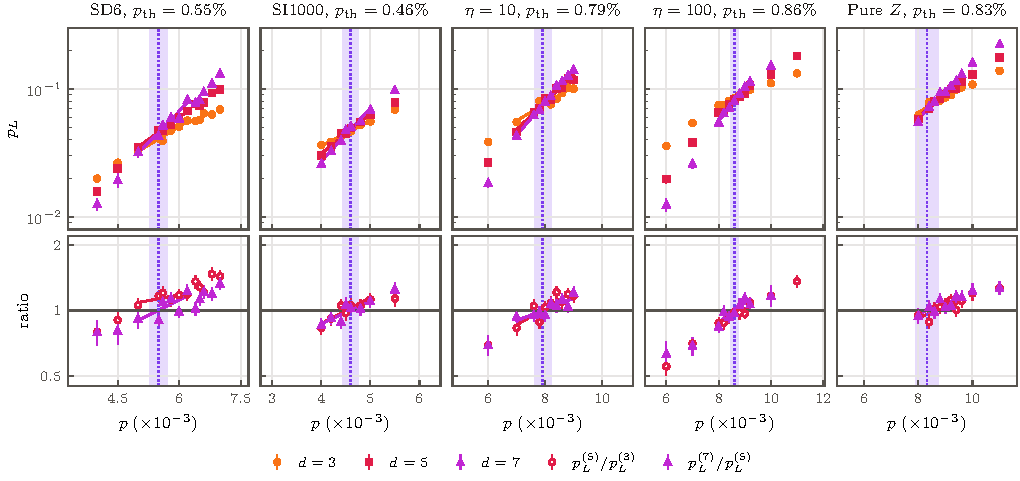
\includegraphics[width=\textwidth]{fig_bm.pdf}
  \caption{Threshold crossings of belief-matching for $r=d$ rounds and $d=3$, $5$ and $7$. Top row, logical error rates with straight-line fits of $\ln\pL$ over $\pm15\%$ around the crossing. Bottom row, ratios of consecutive distances with the ratios of the fitted lines. The vertical line marks the crossing of $d=5$ and $d=7$, where their ratio equals one, and the band its bootstrap uncertainty. Each point near the crossing has between 300 and 650 logical errors.}
  \label{fig:bm}
\end{figure*}

\section{Exact circuit-level fault distance}
\label{app:distance}

We compute the fault distance on the detector error model of the circuit with $\Sz$ detectors. Stim lists every elementary fault together with the detectors and the observable it flips~\cite{gidney2021stim}. Faults with the same detectors and the same observable are merged, which does not change the minimum. Let $H$ be the binary matrix whose columns are the detector sets of the remaining faults and $L$ the row vector of their observable flips. A set of faults, encoded by a binary vector $x$, is an undetectable logical error if
\begin{equation}
  Hx=0 \pmod 2,\qquad Lx=1 \pmod 2 .
\end{equation}
The fault distance is the minimum Hamming weight of such an $x$. We decide whether a solution with weight at most $k$ exists with the CP-SAT solver of OR-Tools~\cite{cpsat}, which supports parity constraints directly. An infeasible instance for $k=d$ together with an explicit solution of weight $d+1$, found either by the solver or by the undetectable-error search of Stim, proves that the fault distance is $d+1$. \autoref{tab:fdapp} lists the instances.

For $d=7$ with seven rounds the solver does not decide the case $k=6$ within one hour, and we use a weaker bound from linear programming. Stim decomposes every fault into at most two edges of the matching graph of the $\Sz$ detectors. Let $w_e\geq0$ be weights on these edges such that the edges of every fault have total weight at most one. The edges of the faults of an undetectable logical error $F$, counted modulo two, form an even subgraph that flips $\Xb$. This subgraph contains a cycle that flips $\Xb$, and the weight of that cycle is at most $|F|$. The minimum weight of a cycle that flips $\Xb$ is therefore a lower bound on the fault distance for every admissible choice of weights. We compute this minimum with shortest paths on the graph that carries the parity of $\Xb$ as an extra label on every vertex, and we maximize it over the weights with a linear program and cutting planes. The bound equals $d$ for $d=3$, $5$ and $7$. For $d=7$ with seven rounds it shows that the fault distance is at least seven, and the search of Stim finds an undetectable logical error with eight faults.

\begin{table}[t]
  \caption{Circuit-level fault distance. For each instance CP-SAT proved that no undetectable logical error with fewer faults exists and found one with the listed number of faults. For $d=7$ with seven rounds the lower bound comes from the linear program of the text and the upper bound from the search of Stim. Mechanisms counts the distinct fault mechanisms of the detector error model. The $\ket{+}^{\otimes n}$ start uses all generator detectors.}
  \label{tab:fdapp}
  \begin{ruledtabular}
  \begin{tabular}{cccccc}
    $d$ & $r$ & Start & Readout & Mechanisms & Fault distance \\
    \hline
    3 & 1 & frame & frame & 51 & 4 \\
    3 & 1 & frame & ideal & 51 & 4 \\
    3 & 3 & frame & frame & 125 & 4 \\
    3 & 3 & frame & ideal & 125 & 4 \\
    5 & 1 & frame & frame & 153 & 6 \\
    5 & 1 & frame & ideal & 153 & 6 \\
    5 & 5 & frame & frame & 613 & 6 \\
    5 & 5 & frame & ideal & 613 & 6 \\
    7 & 1 & frame & frame & 311 & 8 \\
    7 & 7 & frame & frame & 1733 & 7 or 8 \\
    3 & 3 & $\ket{+}^{\otimes n}$ & frame & 465 & 2 \\
    5 & 5 & $\ket{+}^{\otimes n}$ & frame & 3309 & 2 \\
  \end{tabular}
  \end{ruledtabular}
\end{table}

\section{Enumeration of extraction schedules}
\label{app:schedule}

A translation-invariant schedule assigns a layer in $\{1,\dots,6\}$ to each of the six positions of a class-A hexagon and of a class-B hexagon, and two layers to the gates of each link, one value for even blocks and one for odd blocks. Boundary checks use the layers of their cells. A schedule is valid when it satisfies the following conditions:
\begin{enumerate}
  \item No data qubit takes part in two gates in the same layer, and no ancilla is used twice in a layer.
  \item For every pair of overlapping checks, the number of shared qubits on which the two checks apply anticommuting Paulis and the first check acts earlier is even.
\end{enumerate}
The second condition guarantees that the interleaved circuit measures the intended commuting operators. Both conditions are local, so it suffices to check them on a patch that contains every type of overlap. We found 8928 valid schedules. For each we built the $d=3$ protocol with three rounds and computed its fault distance with the undetectable-error search of Stim, exploring all detection-event sets of size at most five. \autoref{fig:schedule}(d) shows the distribution. The schedule used in this paper is one of the 1126 schedules with fault distance four. Its layers are listed in \autoref{tab:schedule}.

\begin{table}[t]
  \caption{Layer of each hexagon position in the selected schedule. The positions are top (T), upper right (UR), lower right (LR), bottom (B), lower left (LL) and upper left (UL). Link gates act on the upper vertex in layer 1 and on the lower vertex in layer 2 for every block.}
  \label{tab:schedule}
  \begin{ruledtabular}
  \begin{tabular}{lcccccc}
    Position & T & UR & LR & B & LL & UL \\
    Pauli & $X$ & $Y$ & $Z$ & $X$ & $Y$ & $Z$ \\
    \hline
    Class A & 1 & 3 & 5 & 6 & 4 & 2 \\
    Class B & 1 & 2 & 3 & 4 & 6 & 5 \\
  \end{tabular}
  \end{ruledtabular}
\end{table}

\section{Threshold fits}
\label{app:fits}

\autoref{tab:fits} lists the parameters of the finite-size scaling fits of \autoref{eq:fss}. For belief-matching we have data for $d=3$, $5$ and $7$ only, with points spaced by $2\%$ to $3\%$ of the threshold around each crossing. We fit $\ln\pL$ of each distance by a straight line in $p$ over $\pm15\%$ of the crossing and quote the point where the lines of $d=5$ and $d=7$ meet, with a bootstrap uncertainty. \autoref{fig:bm} shows these data together with the fitted lines. The crossing of $d=3$ and $d=5$ lies $12\%$ lower under SD6 noise, within the uncertainty for SI1000 and $\eta=10$, and $3\%$ to $5\%$ higher for $\eta=100$ and pure $Z$ noise. The belief-matching thresholds therefore carry a finite-size uncertainty of a few percent beyond the statistical one.

\begin{table}[t]
  \caption{Finite-size scaling fits of \autoref{eq:fss} with $d=5$, $7$ and $9$. $\nu$ is the fitted exponent and $\chi^2_r$ the reduced chi-square. Each fit uses between 18 and 36 data points.}
  \label{tab:fits}
  \setlength{\tabcolsep}{4pt}
  \begin{ruledtabular}
  \begin{tabular}{lcccccc}
    & \multicolumn{2}{c}{MWPM} & \multicolumn{2}{c}{HCM, links} & \multicolumn{2}{c}{HCM} \\
    \cmidrule(lr){2-3}\cmidrule(lr){4-5}\cmidrule(lr){6-7}
    Noise model & $\nu$ & $\chi^2_r$ & $\nu$ & $\chi^2_r$ & $\nu$ & $\chi^2_r$ \\
    \hline
    SD6 & $1.19$ & $0.8$ & $1.23$ & $2.0$ & $1.06$ & $2.3$ \\
    SI1000 & $1.24$ & $1.4$ & $1.09$ & $1.1$ & $1.17$ & $1.2$ \\
    Biased, $\eta=10$ & $1.17$ & $1.7$ & $1.11$ & $1.6$ & $1.07$ & $0.6$ \\
    Biased, $\eta=100$ & $1.12$ & $2.5$ & $1.12$ & $3.3$ & $1.10$ & $0.9$ \\
    Pure $Z$ & $1.25$ & $1.7$ &  &  & $1.03$ & $1.5$ \\
    EM3 & $1.20$ & $2.3$ &  &  & $1.08$ & $1.6$ \\
  \end{tabular}
  \end{ruledtabular}
\end{table}

\autoref{fig:rounds_full} shows the full sweep behind \autoref{fig:rounds_curves}, from $p=2\times10^{-3}$ to $10^{-1}$. Above the threshold window every curve rises to $\pL=1/2$, the value at which the decoder output is uncorrelated with $\Xb$, and no two distances cross again up to $p=10^{-1}$.

\begin{figure*}[t]
  \centering
  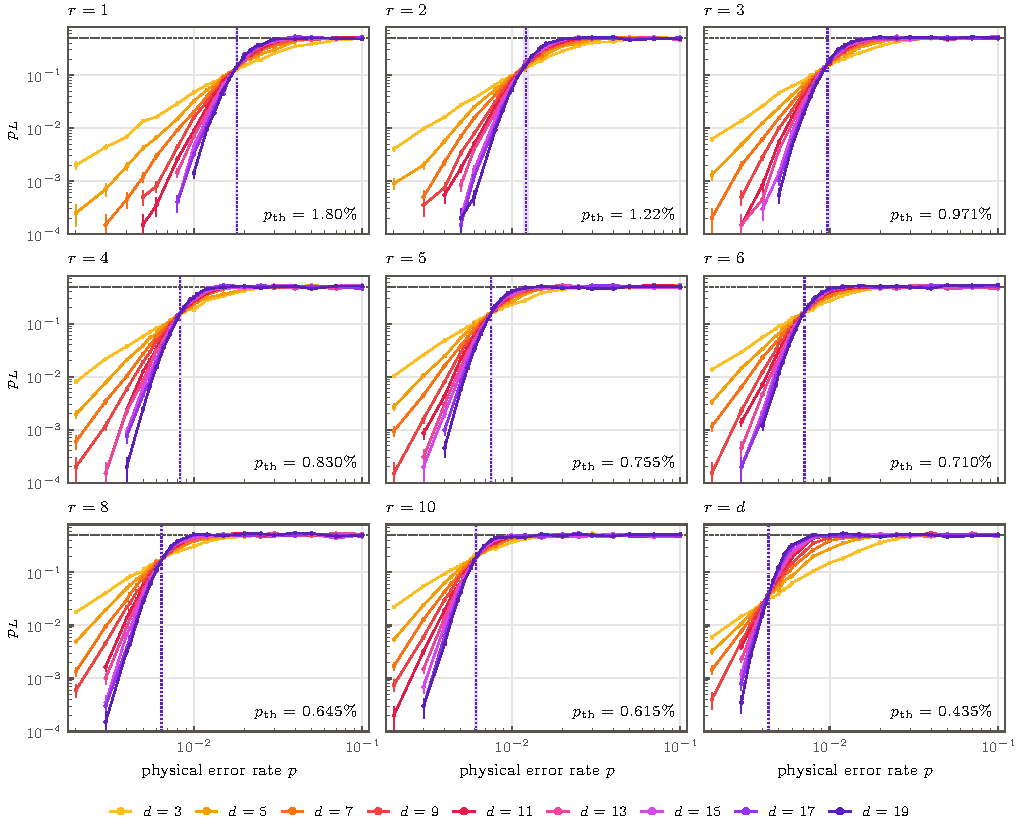
\includegraphics[width=\textwidth]{fig_rounds_full.pdf}
  \caption{Full range of the sweep of \autoref{fig:rounds_curves}, with $d=3$ to $19$ and $p=2\times10^{-3}$ to $10^{-1}$ on logarithmic axes. The dashed line is $\pL=1/2$, and the vertical line and band mark the threshold of \autoref{tab:rounds}.}
  \label{fig:rounds_full}
\end{figure*}


\bibliography{references}

\end{document}
